%                                                                 aa.dem
% AA vers. 9.1, LaTeX class for Astronomy & Astrophysics
% demonstration file
%                                                       (c) EDP Sciences
%-----------------------------------------------------------------------
%
% \documentclass[referee]{aa} % for a referee version
%\documentclass[onecolumn]{aa} % for a paper on 1 column  
%\documentclass[longauth]{aa} % for the long lists of affiliations 
% \documentclass[letter]{aa} % for the letters 
%\documentclass[bibyear]{aa} % if the references are not structured 
%                              according to the author-year natbib style

%
\documentclass{aa}  

%
\usepackage{amsmath}
\usepackage{graphicx, comment}
\usepackage{commath}
\usepackage{txfonts}
\usepackage{subfig}
\usepackage{upgreek}
\usepackage{threeparttable} 
\usepackage{booktabs}
\usepackage{siunitx}
\usepackage{natbib}
\usepackage{float}
\usepackage{enumitem}

% \usepackage[backend=biber, style=authoryear, natbib=true]{biblatex}
% 超链接配置：确保链接颜色可见，去除边框
\usepackage[colorlinks=true, linkcolor=blue, urlcolor=blue, citecolor=blue]{hyperref}
\usepackage{orcidlink}

\newcommand{\C}{3C\,84}
\newcommand{\rotang}{-4.5^\circ}
\newcommand{\protang}{4.5^\circ}
\newcommand{\beam}{(0.17\times0.40)\,\textrm{mas}}

\newcommand{\Mj}{5.0\pm1.7}
\newcommand{\Mjrel}{6.7\pm2.0}
\newcommand{\Mx}{9.8\pm3.2}
\newcommand{\enthalpy}{0.26\pm0.20}
\newcommand{\ajj}{0.14\pm0.06}
\newcommand{\ax}{0.07\pm0.02}
\newcommand{\bw}{0.27\pm0.04}

\newcommand{\rj}{0.36\pm0.09\,\textrm{pc}}
\newcommand{\phij}{4.5^\circ\pm1.2^\circ}
\newcommand{\thetaj}{35^\circ\pm5^\circ}
\newcommand{\gj}{1.35\pm0.14}


\newcommand{\tp}{30\pm10\,\textrm{years}}
\newcommand{\chiamp}{\sim1}
\newcommand{\chialt}{\sim2}




\begin{document} 

\renewcommand{\arraystretch}{1.5}
   
    \title{
    % 1.4GHz下对低红移射电星系的统计：用多种视角观察射电星系的特性
    Topic: \\Paper Name 
    }

    \author{
        P.-G. Zheng\inst{1,2}
    \and R.-Y. Ma\inst{1,2}\thanks{Corresponding author: \email{ryma@xmu.edu.cn}}
    \and Z.-H. Zhu\inst{3,2}\thanks{Corresponding author: \email{}}
    \and X. Cao\inst{1,2}
    \and Y. Xie\inst{4}\thanks{Corresponding author: \email{xieyi@jmu.edu.cn}}
    \and X.-L. Wang\inst{1,2}
    }
    
    \institute{
    Department of Astronomy and Institute of Theoretical Physics and Astrophysics, Xiamen University, Xiamen, Fujian 361005, China
    \and
    SHAO--XMU Joint Center for Astrophysics, Xiamen, Fujian 361005, China
    \and
    Shanghai Astronomical Observatory, Chinese Academy of Sciences, 80 Nandan Road, Shanghai 200030, China
    \and
    School of Science, Jimei University, Xiamen 361021, Fujian Province, China
    }




   \date{Received -; accepted -}


 \abstract
   {
   Radio Galaxies (RGs) are critical active galaxies driving cosmic structure evolution, with jet lobes as key components shaped by interactions with the circumgalactic medium. This study focuses on extracting morphological parameters of Fanaroff-Riley (FR)\textemdash classified RGs (FRI and FRII) from 1.4 GHz radio images via elliptical structure fitting, aiming to systematically characterize their morphological properties. To achieve this objective, a semi-automated workflow is developed to localize RG cores and lobes. Statistical analyses of the derived parameters reveal that both FRIs and FRIIs exhibit a peak axial ratio of approximately 0.25. Notably, FRII RGs possess larger intrinsic physical scales, with the scale distribution peaking at ~200 kpc, whereas the peak scale of FRIs is ~50 kpc. For FRI RGs, the number of knot structures shows a steady decreasing trend within specific brightness intervals. For FRII RGs, a distinct subclass structure emerges in the classification parameter space when $(r_s < 0.4)$, which is attributed to the regulatory effect of hot spot outflows. Furthermore, the stacked curve of the central line brightness of FRII RGs is consistent with the predicted dynamical evolution model of jet-cocoon expansion. These results validate the effectiveness of elliptical structure fitting in describing RG morphologies and provide critical insights into the intrinsic differences between FRI and FRII types. This work establishes a solid foundation for refining RG classification systems and advancing our understanding of active galactic nucleus (AGN) feedback processes in cosmic evolution. 
   }
 
  

   \keywords{
            Active galactic nuclei; Radio galaxy; Radio astronomy
               }

   \maketitle

   
\section{Introduction}\label{sec:Introduction}
% 介绍RGs重要性
Radio Galaxies (RGs) are active galaxies characterized by radio emission driven by jets with scales ranging from pc to Mpc. Since Cygnus A was among the first discrete cosmic RGs identified \citep{hey_fluctuations_1946}, radio observations have remained crucial for understanding the origin, dynamics, and energetics of RGs \citep{hardcastle_radio_2020}. From the mid-1990s to the present, studies on RGs have matured, and it has become increasingly clear that luminous RGs play a pivotal role in the evolution of galaxies and the formation of large-scale cosmic structures \citep{miley_distant_2008}. Most current observations focus on galactic jets, whose dynamical environment is dominated by the stellar/dark matter potential of the host galaxy and the interstellar medium \citep{blandford_relativistic_2019}. Jet lobes, as the outward extensions of galactic jets, have an environment regulated by the backflow from the jet terminals and the circumgalactic medium, and they constitute a critical component of RGs.

% RGs有很多分类
To understand RGs, it is first necessary to enumerate their observable phenomena. By the same token, \citep{krolik_active_1999} suggested that "the only clear way to define Active Galactic Nuclei (AGN) is operationally; all we can do is to list the observable phenomena we use to find them". AGN are classified into radio-loud and radio-quiet subtypes based on their radio loudness\textemdash a key observational parameter defined as the ratio of radio luminosity to optical luminosity \citep{kellermann_vla_1989,sikora_radio_2007}. These radio-loud source is so complex that Fanaroff and Riley (FR) proposed the earliest structural classification of RGs from FRI and FRII, and provided the most fundamental entry point for subsequent research on jet structures \citep{fanaroff_morphology_1974}. However, RGs also possess other classification schemes that are worthy of discussion. In terms of the extended structure of RGs, \cite{owen_ccd_1989} classified RGs into three types based on their radio morphologies: Classical Double sources, Fat Double sources, and Twin Jet sources. Similarly, in terms of their spectra, \cite{osterbrock_broad_1975} categorized RGs into two classes: those with broad permitted emission lines and those dominated by narrow emission lines. Moreover AGN were separated into Seyferts and Low Ionization Nuclear Emission-line Regions \citep{heckman_optical_1980}, and now the diagnostic diagrams is defined to confirm type of RGs \citep{veilleux_spectral_1987}. \cite{laing_spectrophotometry_1994} had divided the narrow-line spectra of FRII RGs and defined low and high excitation galaxy. Compared with other classification schemes, the Fanaroff-Riley (FR) classification scheme exhibits superior advantages in terms of the morphology and brightness distribution of RGs.

% FR的分类也很复杂
However, even the concise FR classification scheme exhibits a certain degree of complexity. \cite{ledlow_20cm_1996} pointed out that while Fanaroff and Riley considered the canonical FRI/FRII luminosity break to be around $L_{150} \sim 10^{26} \si{\watt}\si{\hertz}^{-1}$, the differences between the FRI and FRII forms is not solely a radio power threshold but correlates with the host galaxy's optical luminosity. Classifying lobes as FR types based only on the relative location of the brightness peak within the lobe may be misleading \citep{gopal-krishna_physically-motivated_2023,gasperin_multifrequency_2017}. Nevertheless, the FR classification system exhibits overlaps, such as sources with double-double lobes or HyMoRS, indicating the necessity for deeper understanding beyond traditional FR boundaries \citep{mingo_revisiting_2019,gopal-krishna_extragalactic_2000}. In previous studies, it was generally believed that FRI are low-luminosity RGs characterized by relatively diffuse and poorly collimated jets terminating in diffuse lobes (known as edge-darkened morphology); FRII exhibit well-defined jets that maintain collimation over considerable distances, and these jets typically terminate in bright, well-defined lobes with an edge-brightened morphology. Compared to the FRI type, the newly defined FR0 type has the same core radio luminosity as FRI but hundreds of times less power in the extended emission \citep{baldi_radio_2009,baldi_pilot_2015,baldi_new_2016,baldi_fr0cat_2018}, very similar jets are ejected in both FR classes, but interactions with the environment determine their large-scale morphologies \citep{gopal-krishna_extragalactic_2000}. proposed that FR0, FRI, and FRII LERGs belong to a continuous population \citep{baldi_fr0cat_2018}; it is worth noting that some have observed possible mutual transitions between FRI and FRII types \citep{foschi_evolution_2025,wang_entrainment-limited_2011}. Recently, \cite{fanaroff_new_2021}, utilizing the high sensitivity and resolution of uGMRT and MeerKAT for observations, argued that the FRI/FRII classification remains applicable to the main morphology under high-resolution observations, but requires comprehensive assessment incorporating environmental and detailed characteristics.

% RGs的形态很复杂
% 此段改为对RGs多样性的总结，前面的radio emission内容与RGs结构无关
Since the discovery of diffuse radio emission spanning 1 Mpc in the Coma Cluster in 1959 \citep{large_high-resolution_1959}, subsequent studies have successively initiated observations of the corresponding radio relic. \cite{feretti_clusters_2012} suggested that based on the characteristics of diffuse radio emission, these diffuse RGs can be roughly classified into three types: radio halos, radio mini-halos, and radio relics. But this paper focuses more on the RG structures originating from RGs. The complex mechanisms underpin the emergence of the diverse morphological features of RGs, and some RGs exhibit significant deviations of their jet directions from the initial ones, or their jets undergo a rejuvenation phenomenon, both of which lead to the formation of numerous distorted types of RGs: mirror-symmetric C-shapes and antisymmetric Z-shapes or S-shapes \citep{rudnick_head-tail_1976,florido_spatial_1990,liu_environment_2019}. C-shape RGs can be classified into three distinct morphologies: wide-angle tailed \citep{eilek_what_1984}, narrow-angle tailed  and/or head–tail \citep{lane_3c_2002}. 

% jet机制
To achieve a clear understanding of the geometry of RGs, clarification of the primary mechanisms underlying radio emission from jets is required first. Typically, it is assumed that jets initially begin in a magnetically dominated state, exhibiting a parabolic shape, and reach equipartition where the flow is accelerates magnetically to its terminal velocity, after which the jet transitions to a conical shape \citep{ghisellini_bulk_1989,potter_synchrotron_2013}. In magnetically dominated jets, the operating mechanism is thought to be magnetic reconnection \citep{giannios_role_2006}; in particle-dominated jets, the dominant acceleration mechanism is generally considered shock acceleration \citep{kirk_acceleration_1987}. \cite{agudo_studies_2015} had discussed that during the initial acceleration phase, jets are thought to be Poynting-flux dominated, later transforming into particle-dominated plasma. 


% 前人研究RGs的方法
To establish an understanding of the morphologies of RGs, numerous studies had been conducted as follows: For morphological distinction, \cite{lin_populations_2010} once designed parameters for morphological classification primarily based on the original definition of the FR classification; Subsequently, based on the FR dichotomy, \cite{mingo_revisiting_2019} developed an automated morphological classification tool by quantifying key physical quantities. For specific features, numerous researchers in the past had developed targeted methods to extract features of RGs in specific aspects: Over the past few years, some researchers had mapped both the ridgeline and its brightness distribution by tracing the paths of maximum flux density in radio jets, with the aim of reconstructing the true propagation direction of the jets \citep[e.g.,][]{barkus_application_2021,clews_radio-loud_2025}; Indeed, the concept of ridgeline is not particularly novel, and \cite{velovic_collimation_2022} conducted a detailed analysis demonstrating that ridgeline can elaborate on the information regarding the jet of NGC 2663. Similarly, \cite{bushi_head-tail_2025} divided the radio structure into a number of identically sized circular beam-sized regions, enabling the extraction of quantitative physical information via a standardized framework. \cite{park_discovery_2024,foschi_evolution_2025} had extracted the spine-sheath structure from transverse profiles to investigate the limb-brightened jet morphology. Additionally, there are numerous additional parameters that can be used to characterize RGs, such as the largest angular size \citep[e.g.,][]{vardoulaki_fr-type_2021}, opening angle \citep[e.g.,][]{lao_identification_2025}, and jet pattern \citep[e.g.,][]{ andreasyan_study_2013,javaherian_morphological-based_2023,xie_recognizing_2024}.

% RGs的观测在其他方面的重要性
Observations of RGs possess substantial application potential in other aspects. AGNs play a crucial role in cosmic evolution, with their jets directly mediating AGN interactions\textemdash being assimilated by the circumgalactic medium and terminating in extended radio components where they strongly interact with the surrounding medium via shock waves and instabilities\textemdash yet quantitative measures of this role remain highly uncertain \citep{begelman_theory_1984,blandford_relativistic_2019}. RGs' morphology can further aid in analyzing the activities of the host galaxy, with the most prominent cases being galaxy mergers \citep[e.g.,][]{merritt_tracing_2002,liu_x-shaped_2004,hardcastle_ngc_2019} or recurrent episodes of AGN activity \citep[e.g.,][]{lara_restarting_1999,saikia_recurrent_2009,kuzmicz_optical_2017}. In addition, the Epoch of Reionization (EoR) is a crucial epoch in the evolution of the universe, meanwhile, detecting the 21 cm line of neutral hydrogen originating from the EoR in the low-frequency radio band is a key method for investigating the EoR \citep{madau_21_1997,tozzi_radio_2000,furlanetto_cosmology_2006}.  Furthermore, in the context of the EoR, subtracting the contribution of the model constructed based on the statistical observational data of RGs in the 1.4 GHz band will facilitate our investigation of the EoR. \citep{di_matteo_radio_2002,di_matteo_21-cm_2004}. 

% 自动化方法很重要
Following an extensive literature review, \cite{mingo_revisiting_2019} highlighted the necessity of automated approaches for the scientific analysis of datasets from modern radio surveys. For instance, the Automated Planet Finder has operated continuously in a near-autonomous mode, with its observing team leveraging a suite of high-level Python scripts to enable autonomous operations \citep{radovan_automated_2014,vogt_apflick_2014}. \cite{gupta_machine_2025} had similarly conducted work on the automated analysis of data from radio surveys. Furthermore, such automation efforts greatly facilitate planetary analysis: while automated algorithms excel at classifying compact, unresolved objects, extended sources remain a key challenge \citep{boyce_hydra_2023,boyce_hydra_2023-1}. Integrating multiple methodologies to conduct semi-automated analysis of extended sources is thus imperative.

The primary objective of this work is to extract geometric parameters of RGs by fitting elliptical structures to characterize their morphology, and to conduct statistical analyses of these geometrically derived parameters\textemdash all of which hold physical significance. The structure of this paper is organized as follows: Section \ref{sec:Data} introduces the datasets utilized in this study and their respective sources. Section \ref{sec:Method} details the algorithms implemented herein and defines the geometric parameters. Section \ref{sec:Result} presents the main results, including incidental findings obtained during the execution of the algorithms. Section \ref{sec:Discussion} identifies biases associated with the proposed method and discusses the scientific implications of the results. Finally, Section \ref{sec:Conclusions and Future} provides a comprehensive summary of this work and outlines potential future research directions.
For this paper, we have used a Lambda cold dark matter ($ \Lambda\text{CDM} $) cosmology model for the Universe with Hubble constant $H_{0}$ = 67.74 km/s/Mpc , $\Omega_m$ = 0.3089 and $\Omega_\Lambda$ = 0.6911 based on Planck measurements \citep{collaboration_planck_2016}.




\section{Data}\label{sec:Data}

The image data are sourced from \cite{griese_floriangrieseradiogalaxydataset_2022}, which comprises 2,158 images in total with the following class distribution: FRI (495 samples), FRII (924 samples), Compact (391 samples), and Bent (348 samples). Meanwhile, the processing methods applied to this dataset are detailed in \cite{griese_first_2023}; notably, the dataset provides annotated samples that had undergone preprocessing steps—including denoising and cropping\textemdash to ensure data quality\footnote{\url{https://github.com/floriangriese/RadioGalaxyDataset}}. The dataset come from the Faint Images of the Radio Sky at Twenty-centimeters (FIRST), and all detailed information pertaining to this study in the following sections of the manuscript is derived from the official VLA FIRST Survey website \footnote{\url{https://sundog.stsci.edu/}}. The FIRST survey achieves a detection sensitivity of 1 mJy at 20 cm. While this enables the observation of finer-scale structures compared to the NRAO VLA Sky Survey\textemdash which has a sensitivity of 2.5 mJy\textemdash it exhibits a slight deficit in flux density at levels between 2.0 and 20 mJy \citep{helfand_last_2015}. This deficit is likely attributed to the diffuse flux from extended sources, which is caused of the FIRST beam. In fact, the model proposed by \citep{shabala_delayed_2017} suggests that the actual sizes of AGN-inflated radio lobes may be much larger, but these are too faint to be detected in existing observations.


To obtain galaxy-associated data that matches the positional coordinates of RGs, queries may be conducted via the VizieR\footnote{\url{https://vizier.cds.unistra.fr/}} astronomical data service. Considering the pixel scale of the FIRST telescope snapshot images (where one pixel corresponds to 1.8\arcsec), and the fact that the selected central position might be offset within the surrounding pixel region, a search radius of 5\arcsec was adopted to identify the corresponding galaxies. In the NASA/IPAC Extragalactic Database (NED)\footnote{\url{https://ned.ipac.caltech.edu/}}, optical counterparts near RGs can be systematically searched to locate the RG center and retrieve relevant optical characterization data. However, the discrepancy in the identification of optical counterparts remains notably large. For context, documentation on the official VLA FIRST Survey website notes that approximately 15\% of the sources possess optical counterparts at the detection limit of the POSS I plates. Consistent with this challenge, \citep{helfand_last_2015} noted a significant issue of FIRST in optical counterpart matching and argued that this task poses considerable difficulties. In fact, the method for finding optical counterparts in this work also faces some problems, which will be discussed in \autoref{sec:Discussion}.

\label{sec:Data}



\section{Method}\label{sec:Method}

% 介绍一下Method大概的框架
In this section, a preliminary overview of the semi-automated workflow employed in establishing the elliptical structures of RGs and the associated parameterization process is provided, which serves to establish a general outline of the work presented in this paper; while subsequent subsections will cover the key details. Specific steps can be found in \autoref{fig:Figure1}. Briefly speaking, the data collected in the first step is filtered in the second step; subsequently, the RGs that meet the filtering criteria have their radio structures located in the third step; and finally, the geometric parameters and physical properties will be extracted in the fourth step. Finally, the extracted elliptical structures are presented in \autoref{fig:Figure2}.

% 在这一方面的方法中，椭圆很重要
Elliptical structures are of considerable significance in morphological discussions. \cite{lin_new_2024} recalibrated the luminosity function for various types of RGs at 150 MHz by elliptical structure, and the power spectra of his model are closely aligned with those from the SKADS model. And ellipticity characterizes the distribution of the ICM at large scales and can be used to estimate how long it will take for the main halo to virialize \citep{ghirardini_erosita_2022}. Some double-lobes of RGs' structure can exhibit a morphologically oriented and elongated elliptical structure (such as Cygnus A \citep{carilli_cygnus_1996}). \cite{begelman_overpressured_1989} once utilized the structure of cocoons of shocked gas to describe the RG Cygnus A, constructing a comprehensive physical framework of "Jet - Cocoon - Surrounding Intergalactic Medium"; within this model, the bow shock surrounding hot spots is naturally described as an elliptical structure. In 3C 444, an elliptical feature tangent to the lobe exhibiting a temperature jump characteristic is also observed \citep{croston_large-scale_2011}. Throughout previous analyses of RG structures, the recurrent emergence of a simple elliptical structure can be evidently observed. Clearly, an elliptical structure can be used to provide a general description of radio-loud sources, supply parameters and constraints for modeling extragalactic foreground sources, and conduct statistical analyses based on these parameters.


\subsection{Semi-Automated Workflow}\label{sec:Section3_1}
In this subsection, the extraction of RGs parameters through four steps will be introduced.

\begin{description}
    \item[\textbf{\textit{First Step:}}]
    The first step, this work will utilize the preclassified sample set from the \cite{griese_floriangrieseradiogalaxydataset_2022}, relevant information about which has been described in \autoref{sec:Data}.

    \item[\textbf{\textit{Second Step:}}]
    The second step is excluding unsuitable data. The data acquired in \autoref{sec:Data} exhibit certain imperfections, most notably some RGs with extremely low overall brightness: all bright sources in the image appear extremely faint, or extremely bright ones interfere with target RGs' structure. Such images thus need exclusion from the dataset.


    \item[\textbf{\textit{Third Step:}}]
    The third step, locating the structures of RGs. Although annotated FR classification data has been obtained, to analyze it against FRI/FRII characteristics, it is first necessary to differentiate and localize RGs’ cores and lobes. However, before this, it is first necessary to establish their connectivity to characterize the entire RG system. For FR-type RGs, three operations are needed to localize the entire system: identifying the center, searching for RG-associated clumps, and constructing the central axis. Using NED’s search tool, optical counterparts matching coordinates within the snapshot range can be retrieved (Details of the search are in \autoref{sec:Section3_2}). After simple data cleaning, the remaining optical counterpart coordinates (with basic information) are overlaid on RG snapshots, and the most suitable optical counterpart is retained for subsequent steps. Since this process requires optical counterparts to be near RGs, an algorithm to extract RG contours is needed\textemdash for which the Flood-filling algorithm is used (Details of Flood-filling are in \autoref{sec:Section3_3}). Subsequently, considering interference from other celestial objects besides AGN RGs in RG snapshots, the Principal Component Analysis (PCA) is employed to retain the most prominent AGN system in the entire snapshot (Details of PCA are in \autoref{sec:Section3_4}). Using the optical counterpart’s central coordinates and the PCA-derived principal component direction, a straight line is obtained; clumps along this line may be interpreted as undergoing motion influenced by simple shock acceleration processes. However, these clumps cannot be regarded easily as the entire FR system, the structural rationality still requires verification. Thus, the "center line" is suggested as a reference (Details of center line is in \autoref{sec:Section3_5}). The structure of the center line processed can be viewed in \autoref{fig:Figure3}. After filtering out significant deviations, the most complete RG system structures and their corresponding optical counterpart information are retained. However, due to morphological differences between FRI and FRII sources, strategies for locating optical counterparts near their symmetric centers differ: For FRI sources, optical counterparts are confined to the central bright clump; for FRII sources optical counterparts are positioned near the central line. At this point, the core regions and lobe structures of RGs can be clearly distinguished.


    \item[\textbf{\textit{Fourth Step:}}]
    The fourth step, locating the elliptical structure based on the elliptic Gaussian model (Details of elliptic Gaussian model is in \autoref{sec:Section3_6}). Reliable reference structures vary across morphological classes: FRIs possess well-defined bright cores, while in FRIIs' structures only hot spots demonstrate consistent detectability. Here, elliptical Gaussian models can be fitted to separate step-by-step Gaussian components within the RG system: starting with the optimal single Gaussian component fit, then subtracting the portion explained by this component, and continuing the fitting and subtraction process on the residual image; repeating this until at least 95\% of the brightness distribution is covered. Ultimately, based on the two distinct structures of FR, a minimal ellipse that optimally covers the entire RG can be identified. Meanwhile, procedure will also extract the geometric parameters and physical properties of RGs.

\end{description}


\begin{figure*}[!htbp]
    \centering
    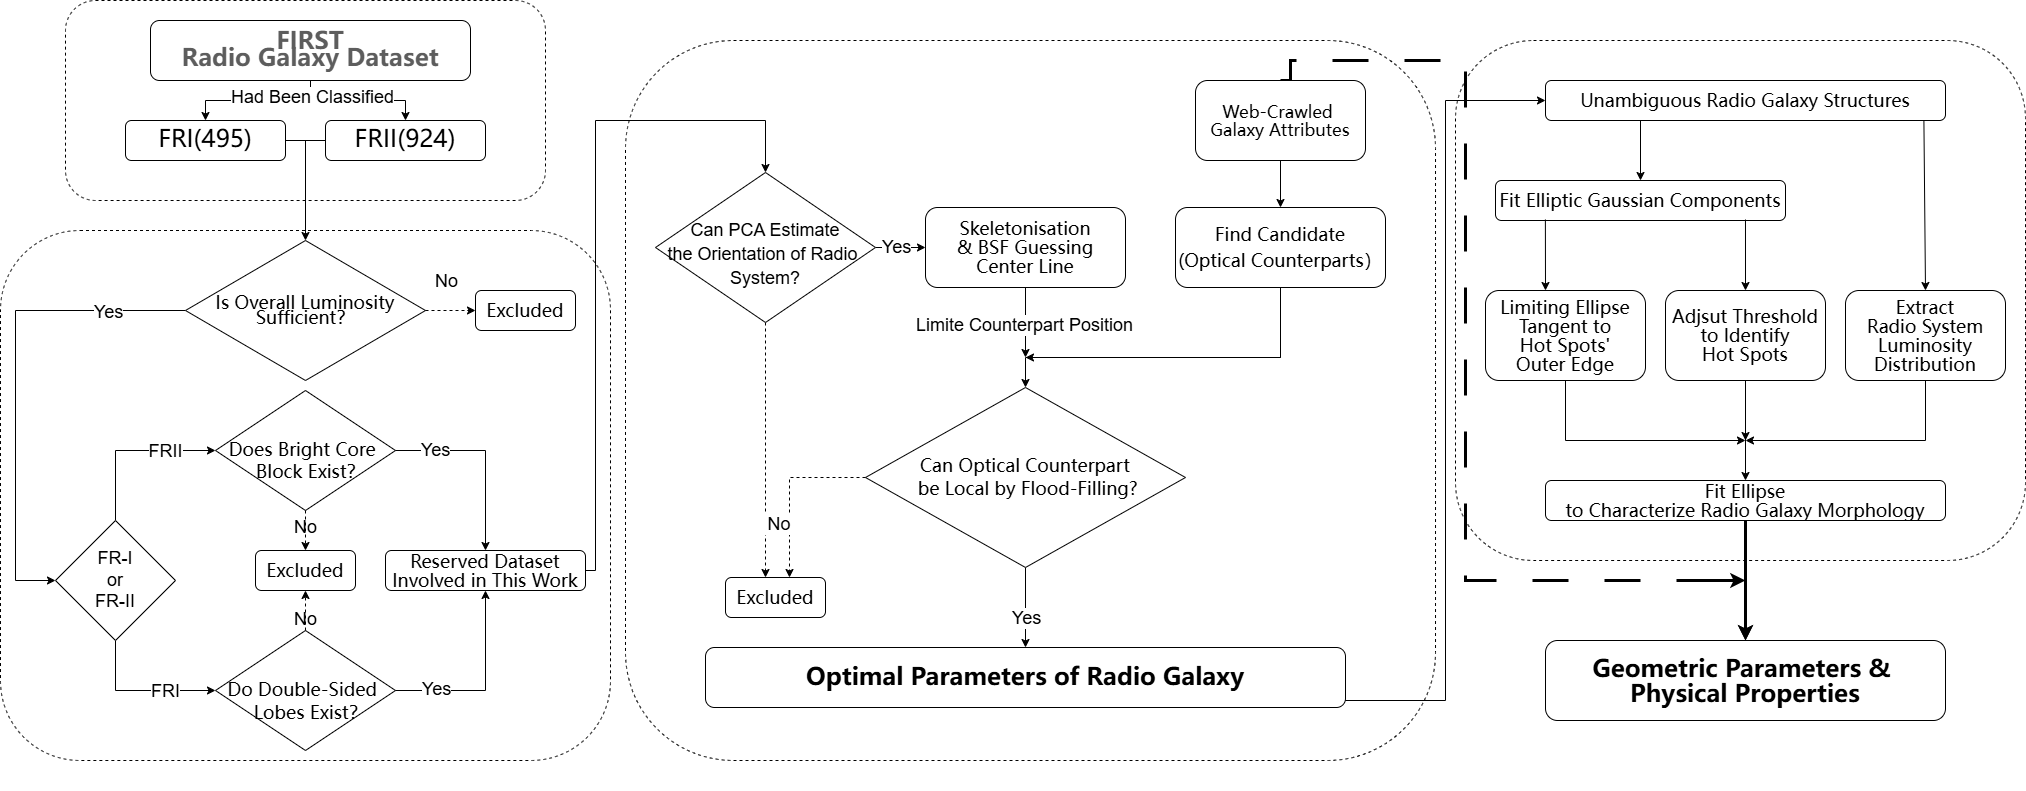
\includegraphics[width=0.9\linewidth]{Figure/Section 3/FR_type_operate.drawio.png}
    \caption{Flowchart for processing FR-classified RGs in \autoref{sec:Method}. The ultimate goal of this job is to conduct statistics on the relevant parameters of the RG.}
    \label{fig:Figure1}
\end{figure*}


\begin{figure}[!htbp]
    \centering
    \includegraphics[clip, trim=105 110 95 90, scale=1.5, width=0.45\linewidth]{Figure/Section 3/244.43_32.384_1_Gendre.png}
    \includegraphics[clip, trim=100 100 100 100, scale=1.5, width=0.45\linewidth]{Figure/Section 3/210.563_23.301_0_MiraBest.png}
    \caption{Left: showing the FRII type source at coordinates (R.A. 244.43°, Dec. 32.384°); Right: showing the FRI type source at coordinates (R.A. 210.563°, Dec. 23.301°).}
    \label{fig:Figure2}
\end{figure}


\subsection{Searching Optical Counterparts}\label{sec:Section3_2}
To position the core of RGs, an effective approach leverages optical host galaxy positional data. For example, when searching for target galaxy-associated sources, \citep{kumar_growth_2022} used NED’s gravitational wave follow-up service to conduct quick-look searches for candidates. Similarly, NED is used here to find optical counterparts and retrieve their data. In \autoref{sec:Section3_1}, the sample’s filtered optical counterparts show redshift distributions (see \autoref{fig:Figure3}), with most redshifts < z=1. Optical counterpart mass and redshift data originate from catalogs archived in Vizier. This becomes challenging when multiple catalogs correspond to one optical counterpart, one catalog includes multiple estimation methods, or both; thus, the average mass is used for individual RGs. Naturally, data with both central black hole and stellar mass measurements is more representative\textemdash entries lacking either were excluded. In \autoref{fig:Figure4}, the central black hole mass and galaxy stellar mass data for FRIs and FRIIs in the sample exhibit a slight degree of misalignment. However, their distribution ranges are so similar that this stands in sharp contrast to the subsequently analyzed parameters with significant differences. This suggests that the mass information observed in the sample may not be the key factor affecting the radio activity of AGNs at 1.4 GHz.

\begin{figure*}[!htbp]
    \centering
    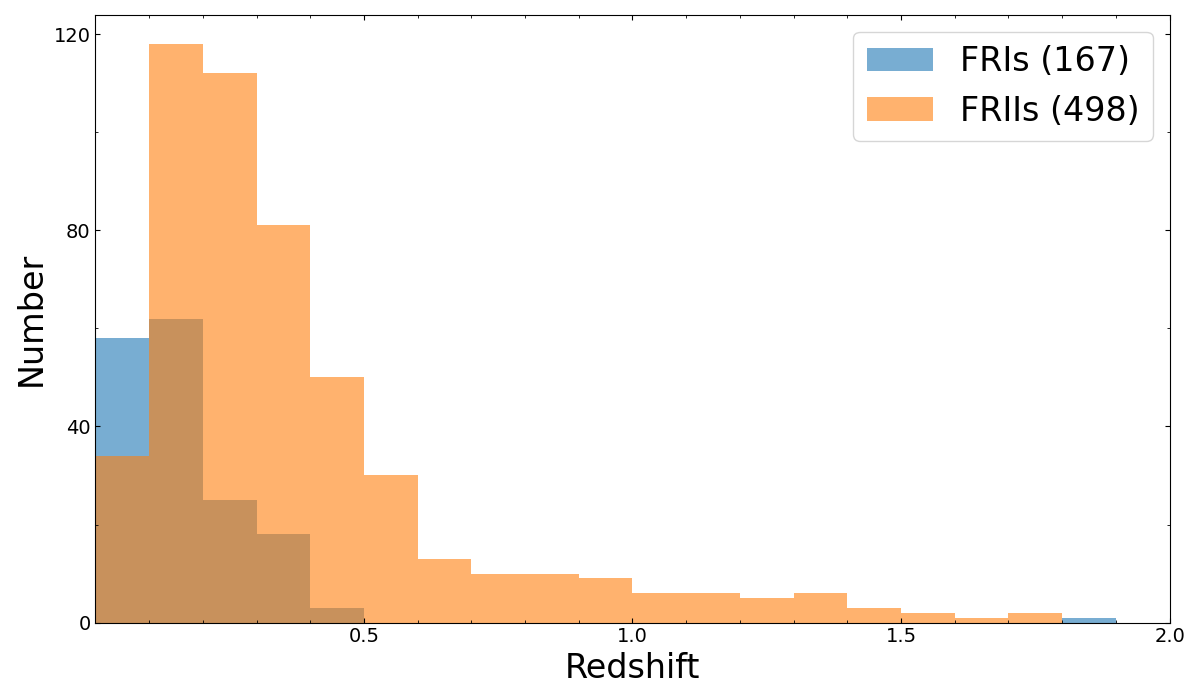
\includegraphics[width=0.9\linewidth]{Figure/Section 3/Redshift.png}
    \caption{Figure 1 presents the redshift distribution of RGs with identifiable optical counterparts selected from the visually screened dataset. The blue histogram corresponds to FRI-type sources, comprising 270 objects, while the red histogram denotes FRII-type sources, with a total of 564 objects.}
    \label{fig:Figure3}
\end{figure*}
\begin{figure*}[!htbp]
    \centering
    \begin{tabular}{cc}
        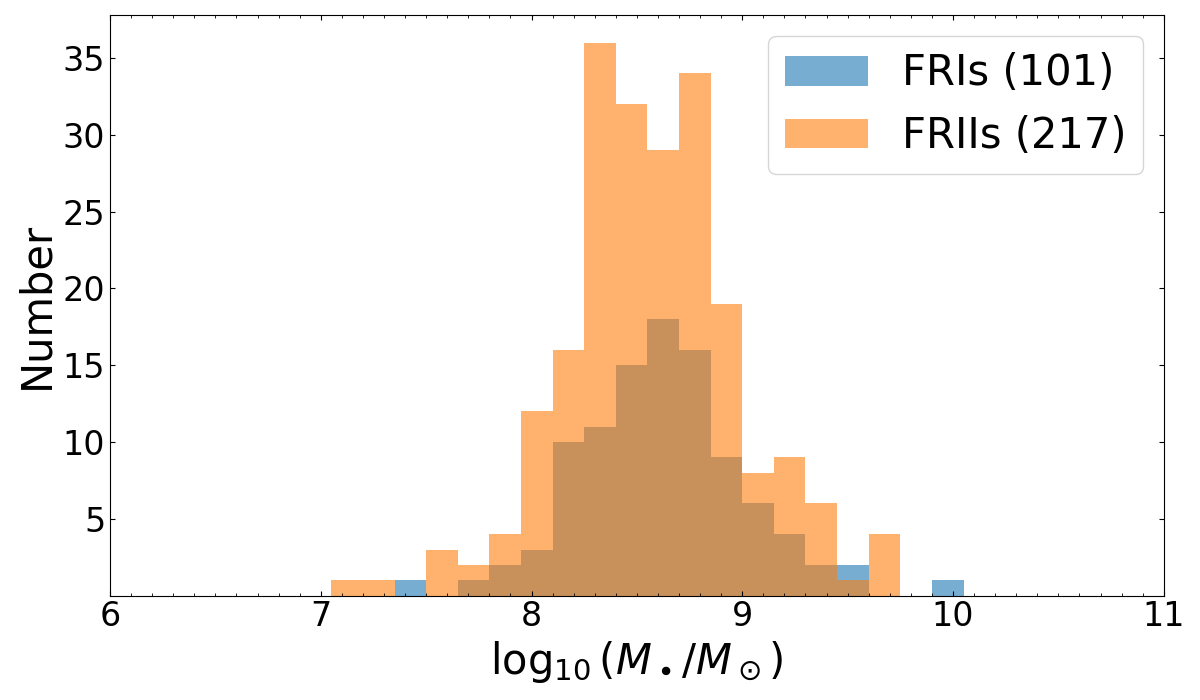
\includegraphics[width=0.45\linewidth]{Figure/Section 3/MassDistribution1.png}&
        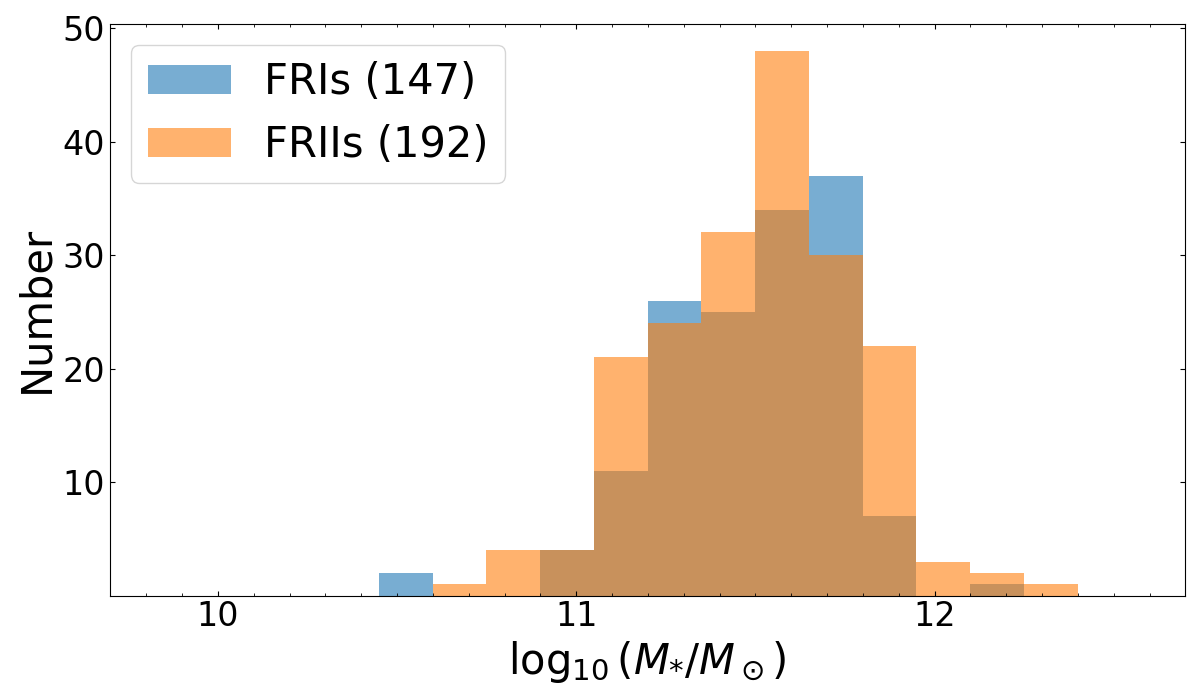
\includegraphics[width=0.45\linewidth]{Figure/Section 3/MassDistribution2.png}
        \end{tabular}
    \caption{The counts distribution plots for central black hole mass (left panel) and galaxy stellar mass (right panel), with the horizontal axis representing the logarithmic value of mass in solar units. In the figure, only the data with a one-to-one correspondence between central black hole mass and galaxy stellar mass are shown (Some optical counterparts may not be found any mass, or only one of them, and they were excluded). All data are the average values derived from the data of designated optical counterparts extracted from VizieR.}
    \label{fig:Figure4}
\end{figure*}


\subsection{Flood-filling Algorithm}\label{sec:Section3_3}
To extract the contours of RGs, employing the Flood-filling algorithm serves as an effective method for determining the extent of the associated RG \citep[e.g.,][]{mingo_revisiting_2019,hales_blobcat_2012}; Starting from known internal points, the Flood-filling algorithm only expands to adjacent non-boundary points, while boundary points are consistently excluded; this facilitates the identification of the contours of RGs under specific conditions \citep{lieberman_how_1978,fishkin_family_1984}. In this procedure, it is specified that the Flood-filling algorithm will disperse seed points in all connected regions of the image with non-zero brightness, while the brightness threshold is set to 5\% of the brightness value of the brightest point in the image.


\subsection{Principal Component Analysis}\label{sec:Section3_4}
Most applications of PCA in astronomy relate to finding eigenvectors across a population of objects, such as PCA tomography \citep[e.g.,][]{steiner_pca_2009}. PCA is a powerful technique for extracting structure from potentially high-dimensional datasets, and a small number of principal components is often sufficient to account for most of the structural information in the data \citep{hofmann_kernel_2008}. Specifically, for the morphological analysis of RGs\textemdash whose observational data typically encompasses multidimensional information (e.g., spatial coordinates and brightness gradients)\textemdash PCA integrates these discrete data points into a low-dimensional principal component space. It prioritizes and preserves the information driven by the highest variance while filtering out noise and redundant signals unrelated to morphology. This enables the direct retrieval of the core morphological features of RGs without relying on complex auxiliary data (e.g., parameters from the Baldwin–Phillips–Terlevich diagram \citep{baldwin_classification_1981}), which aligns with the previously outlined requirement for efficient and concise morphological extraction.


\subsection{Center Line}\label{sec:Section3_5}
Using iterative skeletonization methods, foreground regions can be reduced to single-pixel-wide skeletons while maintaining topological features; for analogous work, see \cite{vardoulaki_fr-type_2021}. For describing the overall orientation of lobe structures, extraneous branches in the skeleton are irrelevant. Thus, the Breadth-First Search algorithm can retain the primary backbone\textemdash most representative of lobe structure\textemdash hereafter referred to as the Center Line. Applying the BFS algorithm alone is insufficient, however: this process requires integrating multiple constraints to ensure the Center Line aligns broadly with the PCA-derived direction and passes through hot spots or other clumps. \cite{barkus_application_2021} implemented similar techniques, though their ridge lines\textemdash designed primarily for identifying and morphologically classifying extended RGs in radio astronomy\textemdash are less suitable for RG systems with large gaps or curved head-tail structures.

\begin{figure*}[!htbp]
    \centering
    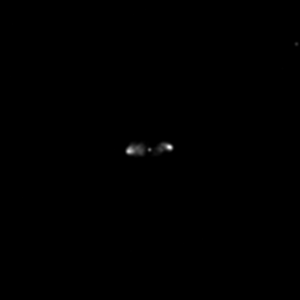
\includegraphics[clip, trim=100 100 100 100, scale=1, width=0.25\linewidth]{Figure/Section 3/178.47_38.197_1_MiraBest.png}
    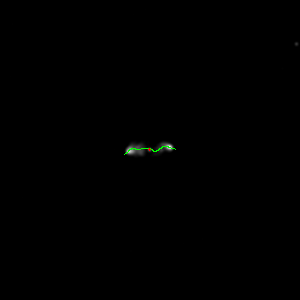
\includegraphics[clip, trim=100 100 100 100, scale=1, width=0.25\linewidth]{Figure/Section 3/CenterLine_178.47_38.197_1_MiraBest.png}
    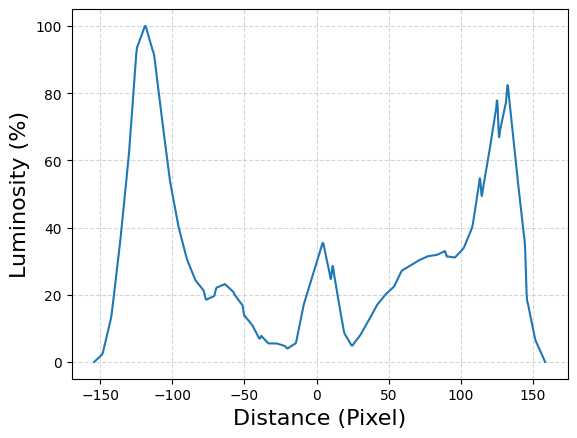
\includegraphics[width=0.33\linewidth]{Figure/Section 3/CenterLineLuminosity_178.47_38.197_1_MiraBest.png}
    \caption{Left: The cleaned RG (R.A. 178.47°, Dec. 38.197°);  Middle: The center line (Green) of RG;  Right: The luminosity distribution of center line.}
    \label{fig:Figure5}
\end{figure*}


\subsection{Elliptic Gaussian Model}\label{sec:Section3_6}

To implement independent modeling of the core region and lobes of RGs, \cite{lin_populations_2010} suggested the angular separation between the highest surface brightness spots on either side of the galaxy as S, and the total linear size of the RG as T, defining $r_s \equiv S/T$ as the primary measure of RG morphology. A critical aspect of this work involves using Gaussian modeling to fit source components; unfortunately, many sources in the dataset employed in this study lack corresponding beam parameters that match those in the FIRST Catalog. 

To ensure the universality of the simulations, their methodology has been simplified: For FRII sources, hot spots are identified by locating the brightest points and outermost elliptical Gaussian components on either side of the optical counterparts of RGs; meanwhile, the maximum distance between the farthest pixels of a RG is adopted as the T value, which characterizes the overall size of the system. For FRI sources, S is defined as the major axis size of the largest elliptical Gaussian component at the system center. For optimal coverage of the entire RG, different strategies are employed based on FR type: For FRI, given its prominent bright core and typical Lobe-Core-Lobe structure, a three-component elliptical Gaussian model is used to fit the central clump and resolve it into one core and two lobes\textemdash with the component assigned the highest brightness weight designated as the core, and the other two as lobes. With the elliptical edges of the two lobes serving as tangent points, a minimal enclosing ellipse is determined. For FRII, an ellipse representing the RG is established using the elliptical Gaussian models of the hot spots: with the principal component direction fixed as the orientation and the elliptical boundaries of the hot spots serving as tangent points, a minimal enclosing ellipse is determined.

The process described above is illustrated in \autoref{fig:Figure6}. And \autoref{fig:Figure2} precisely exhibits the resultant elliptical structure generated after completing these processing steps what are shown in \autoref{fig:Figure1}.

\begin{figure}[!htbp]
    \centering
    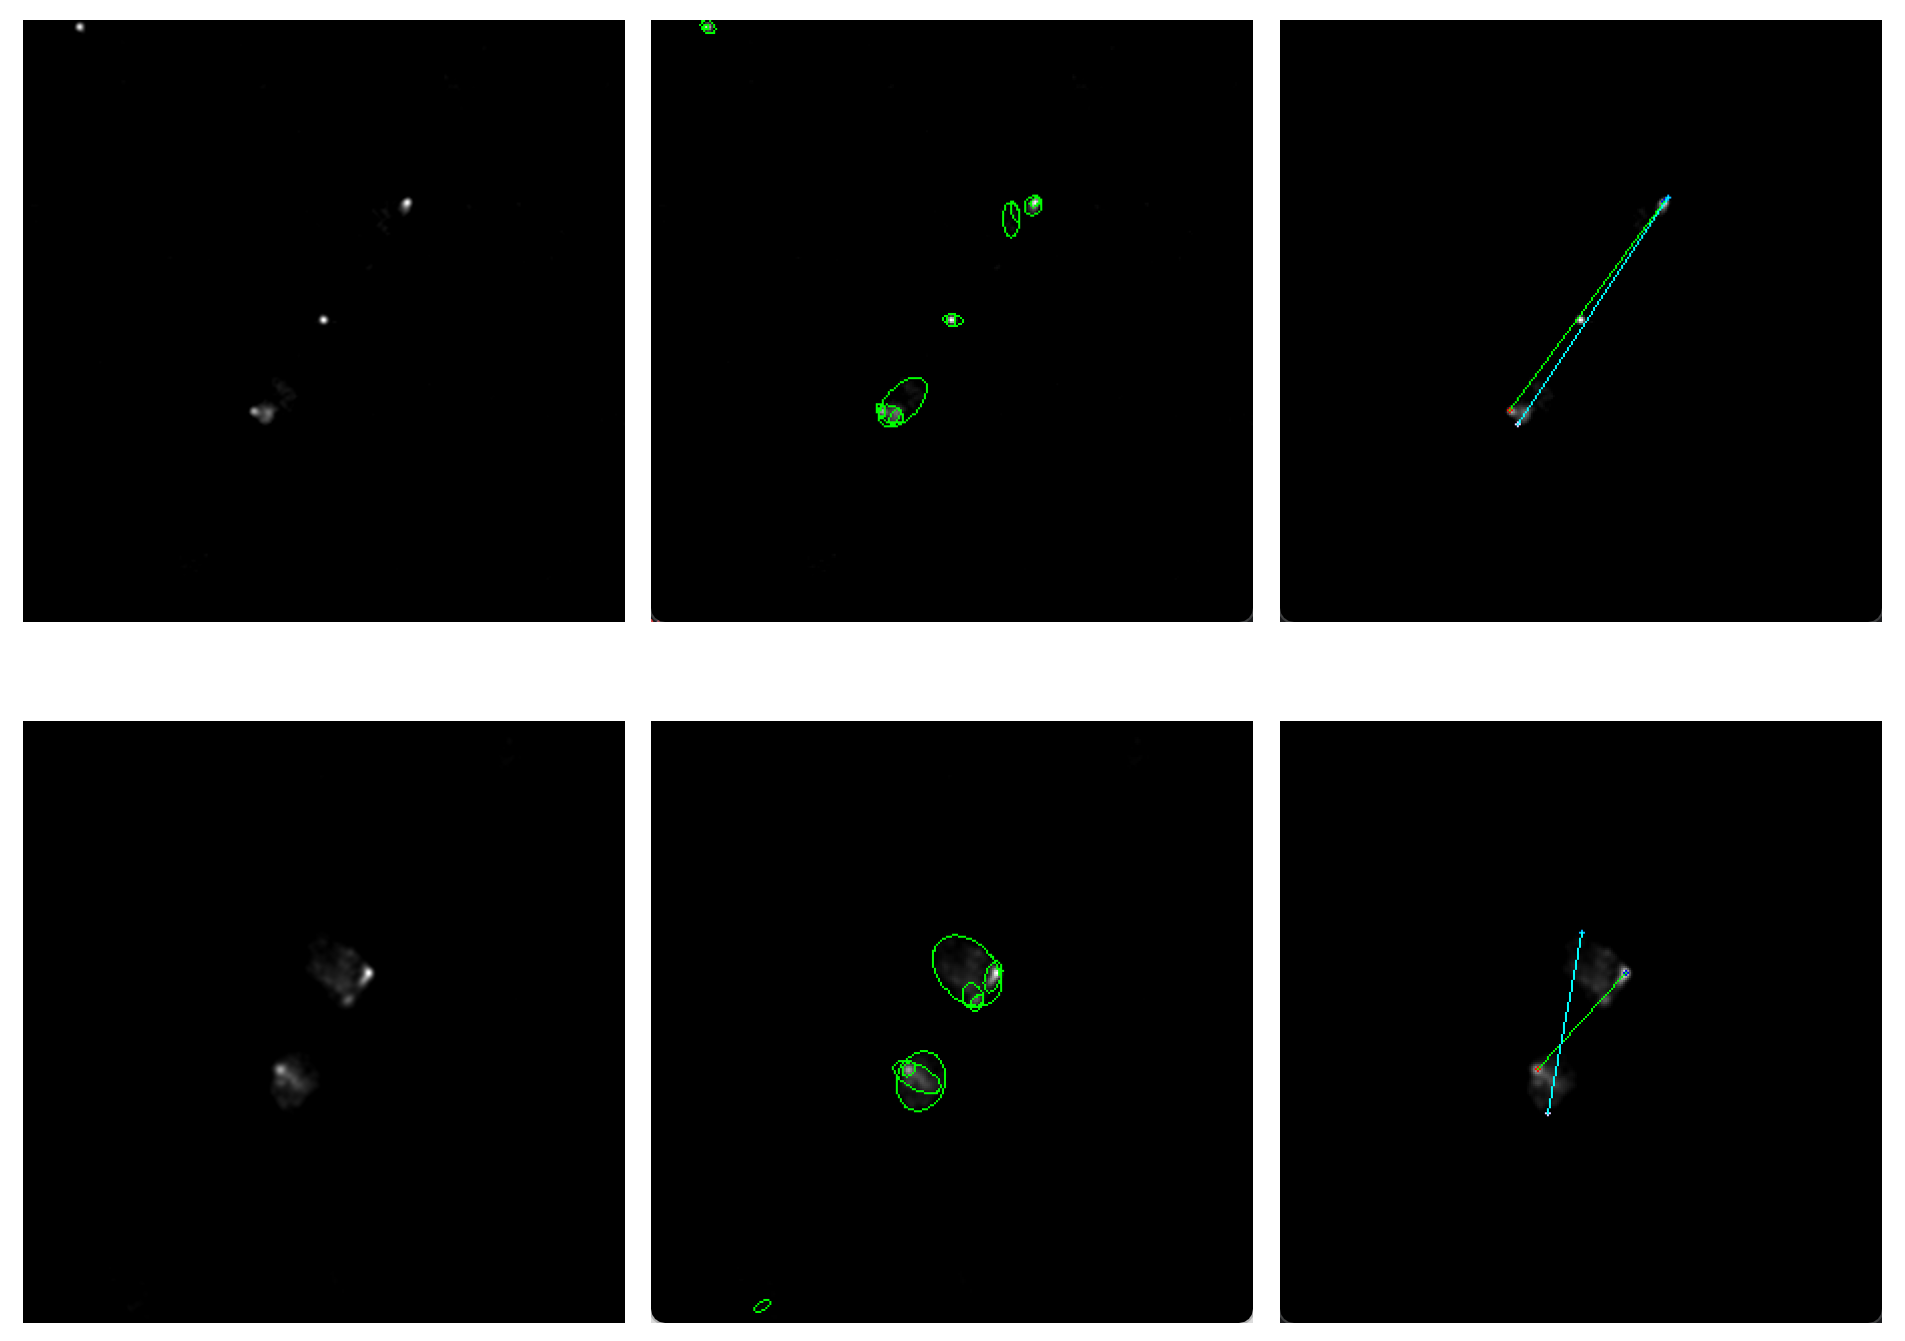
\includegraphics[width=0.9\linewidth]{Figure/Section 3/Different_rs.png}
    \caption{The first column showcases the FRII type source at equatorial coordinates (R.A. 155.486°, Dec. 14.725°), while the second column displays the FRII type source at coordinates (R.A. 148.58°, Dec. 27.267°).}
    \label{fig:Figure6}
\end{figure}


\section{Result}\label{sec:Result}    
\subsection{The Statistical Characteristics of Geometric Parameters}\label{sec:Section4_1}
In \autoref{sec:Section3_6}, elliptical structures can be fitted to FR-type RGs, thereby calculating the axial ratios of these ellipses. \autoref{fig:Figure7} presents binned histograms for FRIs and FRIIs with identical bin counts. In these histograms, a distinct clustering is evident in the FRII distribution—suggesting that FRII radio lobe structures naturally tend to have axial ratios approaching 0.25. Notably, the peak position of FRIs also lies near this 0.25 value.

When locating the principal component direction in \autoref{sec:Section3_1}, this direction can be used to trace the maximum separation distance between the two extremities of the RG system. Given that the optical counterpart has already been localized, its redshift can be determined; this enables the approximate estimation of the RG system’s intrinsic physical scale through corrections based on cosmological models. \autoref{fig:Figure8} shows the distribution of these intrinsic physical scales. The distributions immediately reveal that the physical scales of FRIIs generally exceed those of FRIs: as shown in the subplots, FRIs peak near 50 kpc, while FRIIs exhibit a peak around 200 kpc.

\begin{figure*}[!htbp]
    \centering
    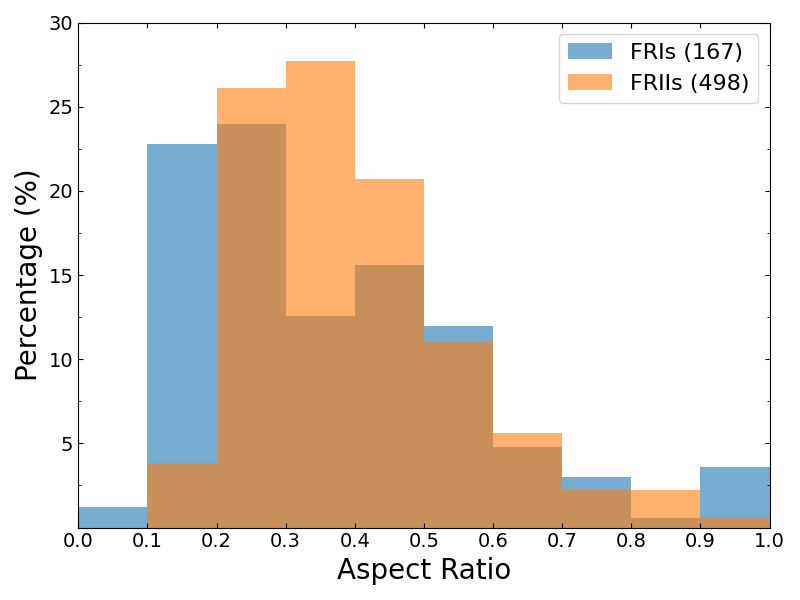
\includegraphics[width=0.9\linewidth]{Figure/Section 4/AxisRatio.png}
    \caption{The vertical axis represents the number of RGs, and the horizontal axis represents the axial ratio of the fitted ellipses. Left Panel: Matching FRIs; Right Panel: Matching FRIIs.}
    \label{fig:Figure7}
\end{figure*}
\begin{figure*}[!htbp]
    \centering
    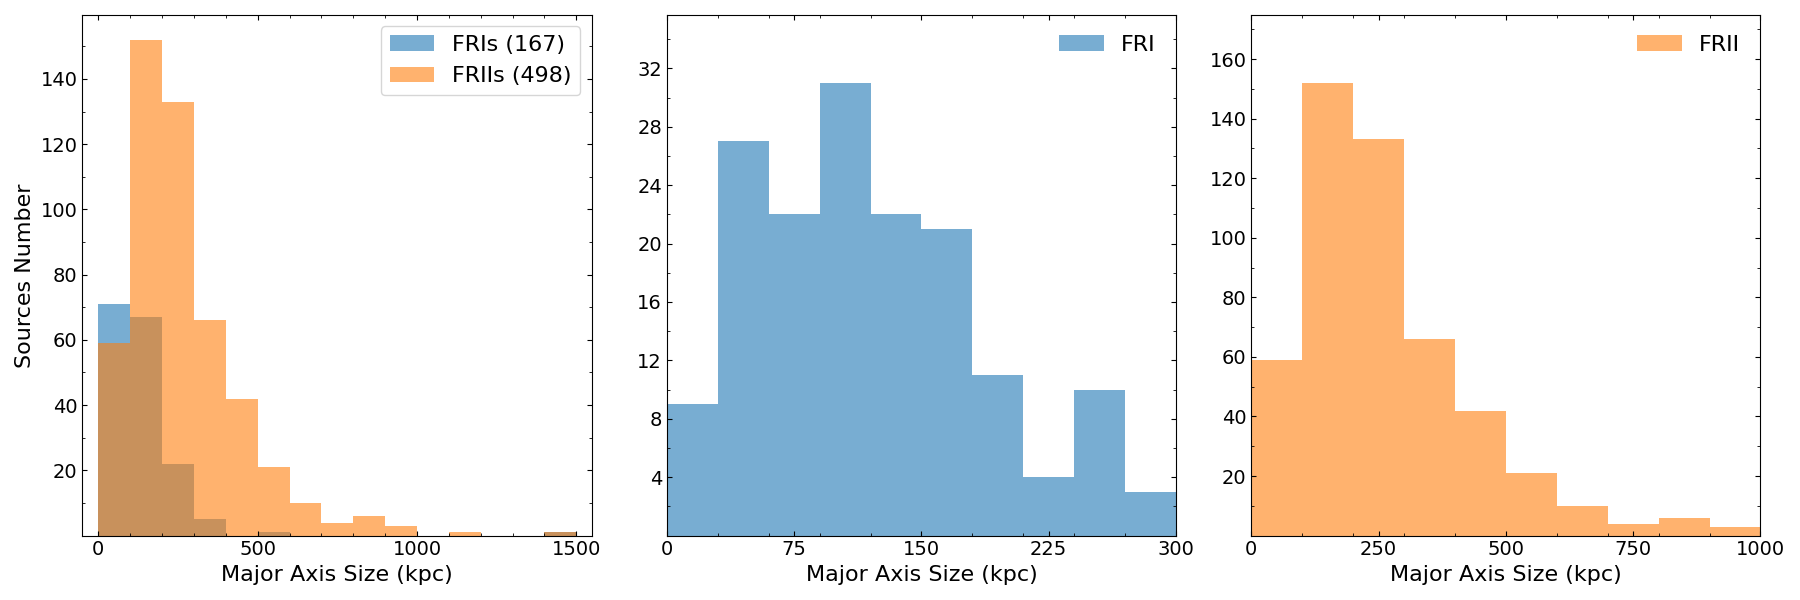
\includegraphics[width=0.9\linewidth]{Figure/Section 4/Max_Scale_Distribution.png}
    \caption{The distribution of intrinsic physical scales of RGs classified by FR type. The blue histogram represents the corrected maximum intrinsic physical scales for FRIs, while the red histogram shows the corrected maximum intrinsic physical scales for FRIIs. The two subplots respectively correspond to enlarged views of the concentration regions of the distributions.}
    \label{fig:Figure8}
\end{figure*}


% Nodes分布特征
\subsection{The Node Structure of FRIs}\label{sec:Section4_2}

\cite{mizuno_recollimation_2015} investigated the mechanism and numerical simulations of jet recollimation: when AGN jets interact with their cosmic environment, they narrow and brighten over a characteristic length scale. During processing in \autoref{sec:Section3_3}, interest in knot structures emerged, leading to the incidental development of a counting method. This method is straightforward: building on the aforementioned flood-filling approach, a threshold (as a percentage of the central clump's maximum brightness) is incrementally increased to constrain the RG extent. Distinct knots are revealed in this process\textemdash with rising thresholds, knots originally blended in lobes gradually separate, then fade, leaving only the bright core (similar to \autoref{fig:Figure9}). A key distinction must be clarified before presenting results: "knot" refers to clumpy structures excluding the bright core in FRI sources, whereas "node" includes the bright core.


As illustrated in the left panel of \autoref{fig:Figure10}, the relationship between RG count and node count is presented, demonstrating that the peak RG count occurs at two nodes with a gradual decrease in RG abundance as the node number increases. When the brightness threshold for Flood-filling is set to a relatively low value (red and green dotted lines), the majority of FRIs exhibit a single massive clump featuring a bright central region and dimmer peripheral segments, with only a negligible fraction presenting extra substructures. As the brightness threshold is moderately elevated (blue dotted line), a subset of FRIs disaggregates into discrete sub-clumps. Subsequently, as the brightness threshold is further increased, the number of sub-clumps per FRI declines, whereas the proportion of FRIs manifesting as a single clump rises. Detailed evolutionary characteristics are elaborated in the right panel.


As illustrated in the right panel of \autoref{fig:Figure10}, three curves of distinct colors depict the number of RGs with different structures as a function of the brightness threshold. Herein, the statistical sample comprises 270 FRIs. Due to the constraints of the flood-filling algorithm implemented in this study, a contour-enclosed area that is excessively small is not recognized as a distinct region. Consequently, prior to the 75\% brightness threshold, a small number of FRIs with near-compact structures induce a slight decline in the black curve. Beyond 75\%, further increases in the brightness threshold result in an increasing number of FRIs retaining only an extremely small bright central region, leading to an accelerated downward trend of the black curve. Meanwhile, the blue curve in the right panel exhibits two primary trends: an accelerated growth in the number of sub-clumps before 10\%, followed by a fluctuating decrease between 10\% and 70\%. In contrast, the cyan curve illustrates that the number of FRIs without substructures drops rapidly before 10\% and fluctuates between 10\% and 70\%. Eventually, driven by the downward trend of the black curve, both the blue and cyan curves experience a combined accelerated decline, and all FRIs eventually evolve into pure nuclear clumps.


\begin{figure*}[!htbp]
    \centering
    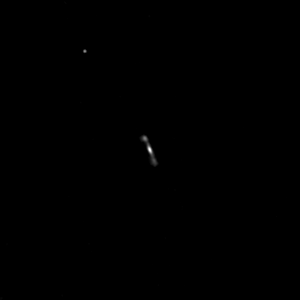
\includegraphics[clip, trim=125 125 125 125, scale=1, width=0.25\linewidth]{Figure/Section 4/Knot_ori.png}
    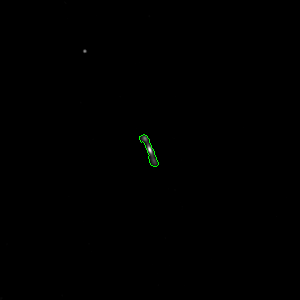
\includegraphics[clip, trim=94 94 94 94, scale=1, width=0.25\linewidth]{Figure/Section 4/Knot_0.5.png}
    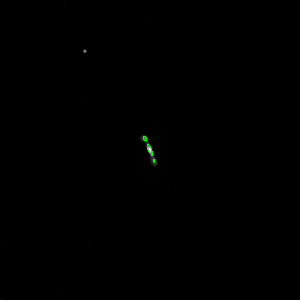
\includegraphics[clip, trim=94 94 94 94, scale=1, width=0.25\linewidth]{Figure/Section 4/Knot_25.png}
    \caption{A FRI type RG located at equatorial coordinates (R.A. 197.092°, Dec. 23.521°). As the threshold increases, four knots are exposed. Left: The original RG (R.A. 178.47°, Dec. 38.197°);  Middle: The contour (Green) of RG;  Right: The contours of clumps when the threshold is 25\%.}
    \label{fig:Figure9}
\end{figure*}

\begin{figure*}[!htbp]
    \centering
    \begin{tabular}{cc}
        \includegraphics[width=0.5\linewidth]{Figure/Section 4/Node_Number.png}& 
        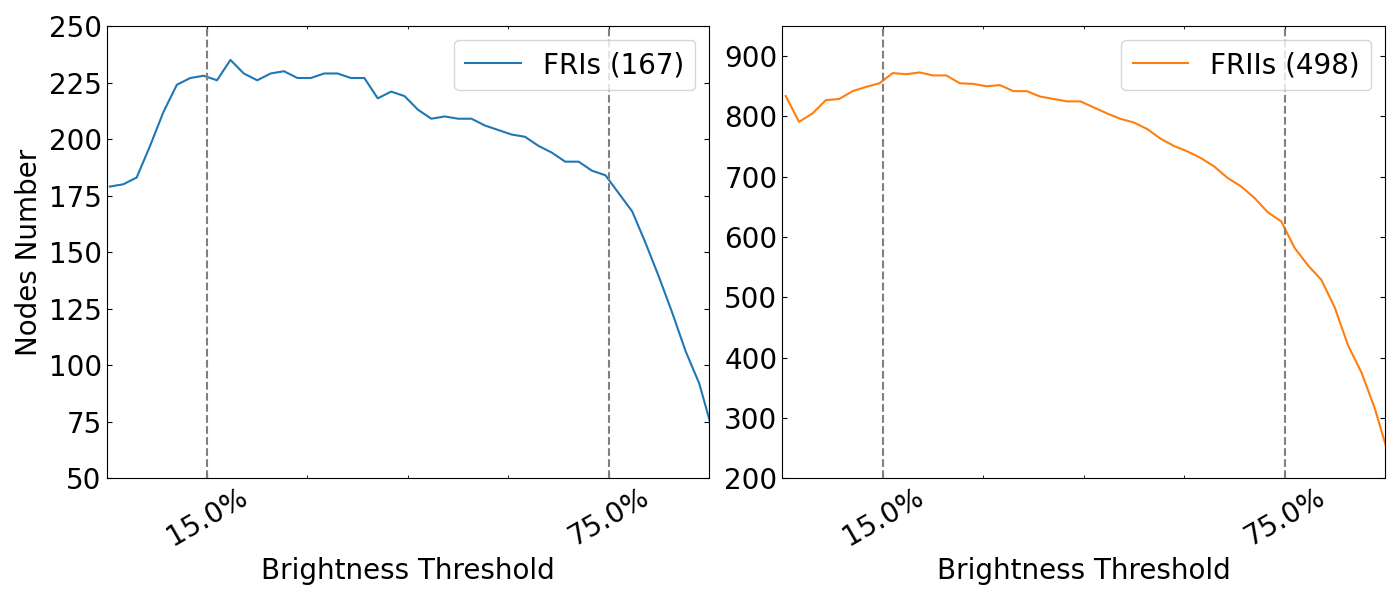
\includegraphics[width=0.45\linewidth]{Figure/Section 4/Node_Evolution.png}\end{tabular}
    \caption{Left Panel: For FRIs, the distribution plot showing the maximum number of nodes appearing as the brightness threshold varies, with the horizontal axis representing the number of nodes and the vertical axis representing the count of RGs possessing that number of nodes; Right Panel: Variation of counts of different types with brightness threshold; The horizontal axis represents the brightness threshold expressed as a percentage of the brightest point in RGs, and the vertical axis denotes the number of RGs or nodes.}\label{fig:Figure10}
\end{figure*}
% \clearpage



\subsection{Classification Parameter $r_s$}\label{sec:Section4_3}

In \autoref{sec:Section3_6}, we reference the methodology for FR-type classification proposed by \cite{lin_populations_2010}, wherein FRIIs exhibit distinct and independent features in the region where $r_s < 0.3$. Building upon this methodology, we identify distinct subclass structures in this region. For $r_s < 0.3$, the distance between the two hot spots is considerably smaller relative to the overall size of the radio structure. However, targeted manual sampling of the dataset in this study reveals that this feature primarily stems from relatively prominent "outflow" structures: clumps centered on the hot spots extend outward in various directions. If such extension does not align with the optical counterpart (or central clump), the algorithm will expand the size of the ellipse to meet the specified coverage rate during fitting, ultimately resulting in a remarkably small hot spot distance relative to the major axis of the ellipse. 

However, is an excessively stringent coverage rate the primary factor affecting the fitting of elliptical Gaussian components for hot spots? In \autoref{fig:Figure12}, it can be observed that even as the coverage level of elliptical Gaussian components decreases incrementally (set at 95\%, 90\%, 80\%, 70\%, 60\%, and 50\%), the subclass structure remains stable. With the reduction of coverage constraints, the faint outflows on both sides of the lobes are the first to be excluded from the ellipses; but, it is evident that they do not significantly affect the stability of the subclass structures.
% FRIs的r_s没很显著的特征，就不展示了——在4.5提出了这件事


% \begin{figure}
%     \centering
%     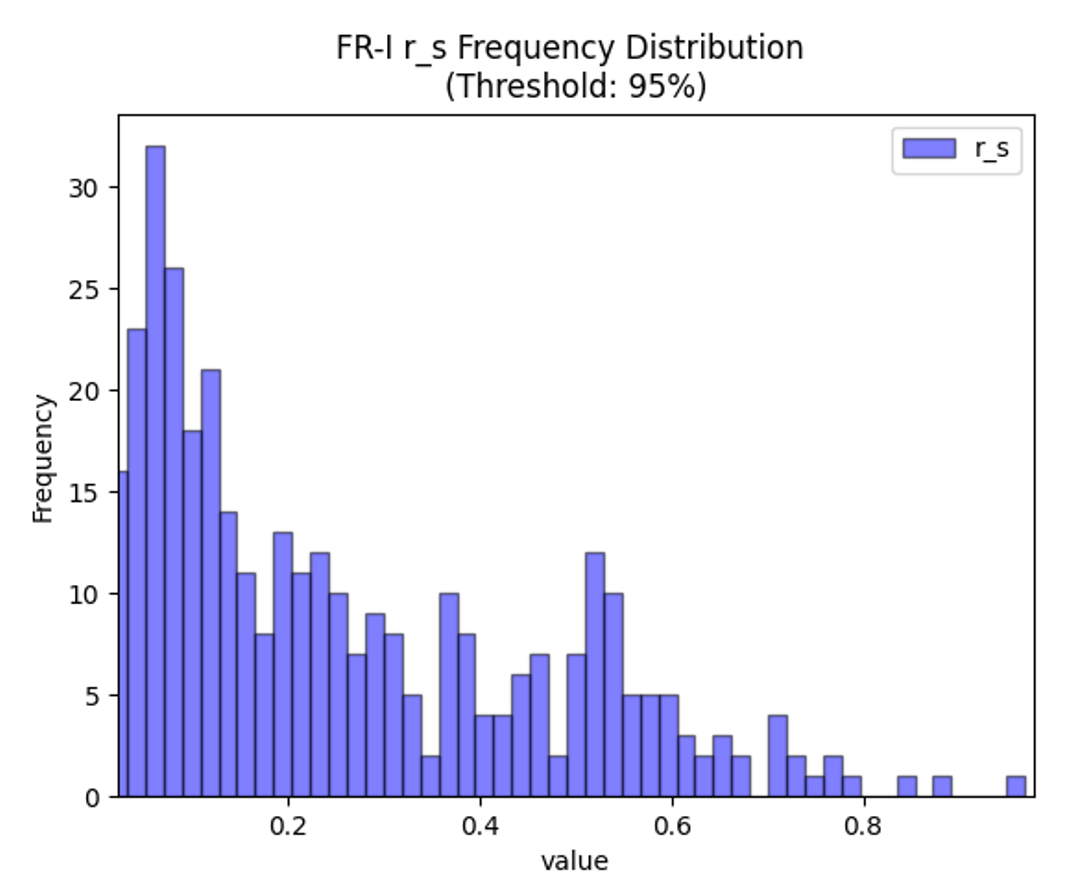
\includegraphics[width=0.9\linewidth]{Figure/Section 4/FR1_rs.png}
%     \caption{Distribution of $r_s$ values for FRIs. The horizontal axis represents the magnitude of $r_s$ values, and the vertical axis denotes the occurrence frequency of RGs corresponding to each $r_s$ value.}
%     \label{fig:Figure11}
% \end{figure}
\begin{figure*}[!htbp]
    \centering
    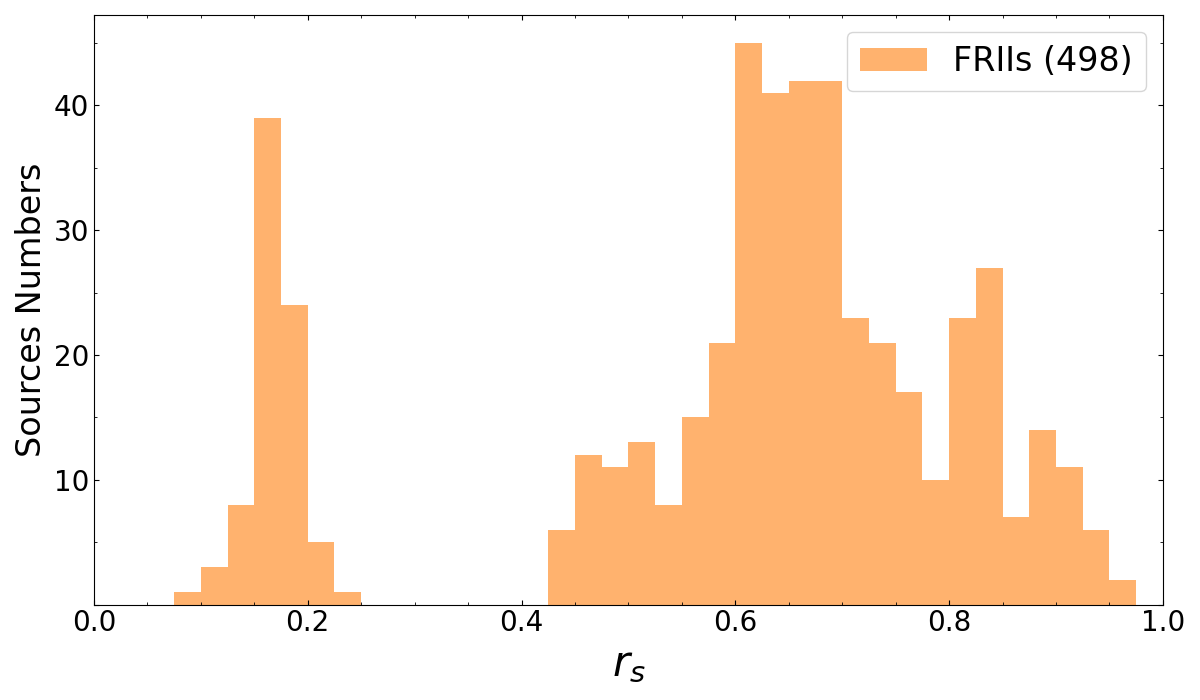
\includegraphics[width=0.45\linewidth]{Figure/Section 4/r_s_distribution0.png}
    \caption{
    Presents the distribution of $r_s$ for brightness thresholds of 95\% (blue) and 50\% (blue, completely obscured by the underlying wine red).
    }
    \label{fig:Figure12}
\end{figure*}
    % 和3D 一起绘制
    % Left Panel: Presents the distribution of $r_s$ for brightness thresholds of 90\% (orange) and 95\% (red, fully obscured by the orange). Right Panel: Presents the distribution of $r_s$ for brightness thresholds of 95\%,90\%,80\%,70\%,60\% and 50\%.



\subsection{The Feature of Center Line Brightness Stacking Curve}\label{sec:Section4_4}

\cite{turner_energetics_2015} previously proposed an evolutionary model for FRI/FRII radio AGNs and their mutual transitions. To reveal the dynamical mechanisms of jet-ambient medium interactions, they developed a comprehensive model that encompasses the supersonic, transonic, and subsonic phases of jet-cocoon expansion, alongside a comparative pure FRII model (where jets maintain supersonic expansion throughout their entire lifecycle). Thus, how can these characteristics be captured? In \autoref{sec:Section3_5}, we propose using the centerline to characterize the brightness distribution of RG. However, constrained by observational resolution, only the most prominent regions can be focused on; nevertheless, stacking these prominent regions may reveal characteristics of the population evolution of FRIIs. To investigate the brightness properties of cores and lobes, the centerline brightness distribution curves of all FRIIs (e.g., \autoref{fig:Figure5}) were acquired.

% 逆推导亮度真实分布
To stack all center lines, the use of standard cosmological models is required for conversion: pixel distances in snapshots are translated to physical scales, and pixel intensities to calibrated luminosity. Given that the image data employed in this work have undergone brightness normalization (scaled to 0–255), it is further necessary to investigate the flux densities of FRIIs to convert pixel brightness into physically meaningful brightness. By means of querying the specified FRIIs in the FIRST catalog via VizieR, combined with previously collected information, an inverse transformation of the work presented in \cite{griese_first_2023} can be performed:
\begin{equation}
\makebox[\linewidth]{$norm\_val = \frac{uint8\_val}{255}.$}
\end{equation}
Two key parameters are defined as follows, \textit{norm\_val} denotes the normalization value, and \textit{uint8\_val} represents an unsigned 8-bit integer value. The flux density in the original images is thus expressed as:
\begin{equation}
\makebox[\linewidth]{$flux\_clip = norm\_val \times (max\_clip - min\_clip) + min\_clip.$}
\end{equation}
Here, \textit{max\_clip} denotes the maximum brightness of the cropped image, derived from the maximum Fpeak retrieved from the 'first14' catalog (VizieR query) with a box size of 9 arcmin (1.8\arcsec  $\times$ 300); \textit{min\_clip} refers to three times the minimum Rms. Given that the brightness units of images from the FIRST survey are 'mJy/beam', the flux\_clip must be converted with the beam size. As proposed in \cite{helfand_last_2015}, the angular area of a single pixel in the image is $(1.8\arcsec)^2$. South of a declination of $+4^\circ 33\arcmin 21\arcsec$, the beam is elliptical with dimensions $6.4\arcsec \times 5.4\arcsec$, where the major axis is aligned north-south. South of a declination of $-2^\circ 30\arcmin 25\arcsec$, the size of the elliptical beam further increases to $6.8\arcsec \times 5.4\arcsec$. Distinguish different situations, the flux of a single pixel \textit{S\_pixel} is expressed as:
\begin{equation}
\makebox[\linewidth]{$S\_pixel = flux\_clip \times \frac{pixel\,size}{beam\,size}.$}
\end{equation}
Based on the formula for calculating the 1.4 GHz radio luminosity \citep{koziel-wierzbowska_identifying_2021} ($\alpha$ is adopted as 0.75, serving as the mean spectral index for sources detected at 1.4 GHz), the luminosity of a single pixel is converted to:
\begin{equation}
\makebox[\linewidth]{$L\_pixel = \frac{4\pi D_L^2}{(1+z)^{1-\alpha}}\,S\_pixel.$}
\end{equation}

To assess the error budget, three factors are considered in this work. First, the FIRST official website specifies a typical rms of 0.15 mJy, while rms values derived from cropped images deviate from this reference. Second, VizieR notes that for bright sources, the accuracy of Fpeak is limited to approximately 5\% due to systematic effects. Third, a code modification for pixel position bias correction is introduced, which simulates pixel position deviations in the calculation of the horizontal axis physical scale to estimate errors caused by pixel discretization. However, minor deviations from redshift and cosmological models are not considered. Additionally, the error propagation formula is applied to each calculation step. Finally, red shaded regions are used to represent the errors in \autoref{fig:Figure13}.
% 最终换算出来的单个RG最大光度范围大概是 1e28-1e32 W/Hz 居多，是否存在问题？


In the present work, we seek to verify Turner’s conclusions. Specifically, we split the center lines of FRIIs at their optical counterparts\textemdash thereby doubling the sample size\textemdash and then stacked the brightness distributions of all sample central lines, from which we derived the brightness stacking curve presented in \autoref{fig:Figure13}. The statistically derived brightness-stacked profiles of FRIIs exhibit structural similarity to their luminosity-size profiles: within 100 kpc of the optical counterpart, the brightness increases with distance until reaching a peak, followed by a steep decline where brightness decreases rapidly with increasing distance. Notably, the FRIs' population did not exhibit significant characteristics and thus are not presented herein.



\begin{figure*}
    \centering
    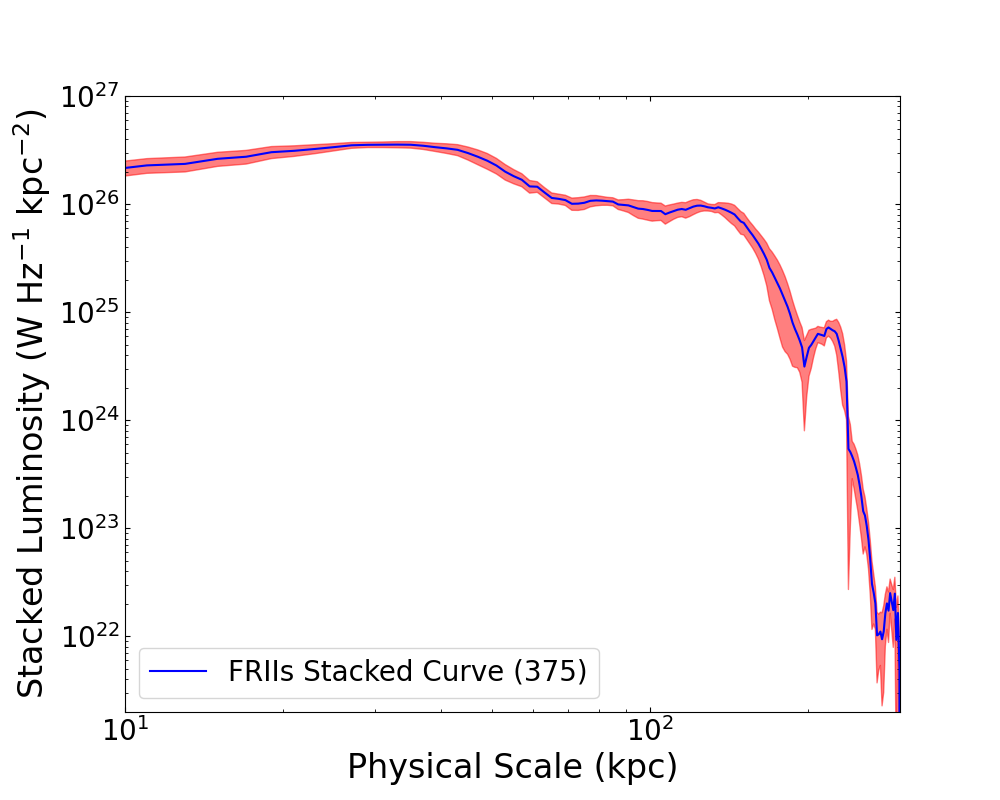
\includegraphics[width=0.45\linewidth]{Figure/Section 4/FR2_StackingCurve1.png}
    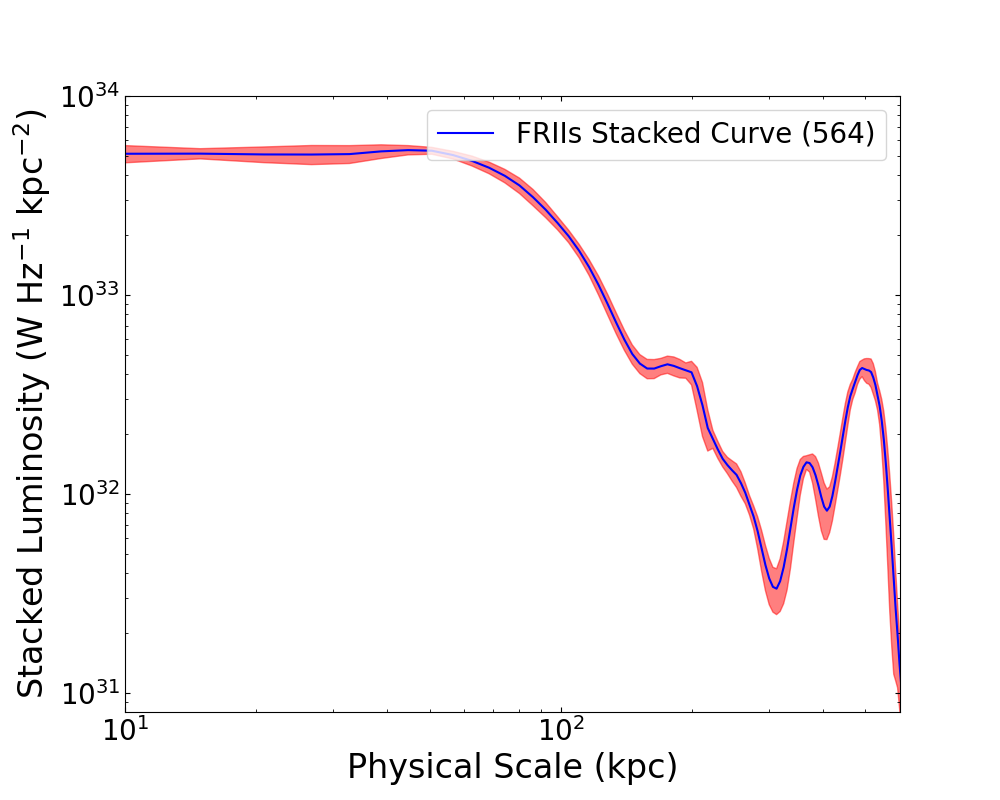
\includegraphics[width=0.45\linewidth]{Figure/Section 4/FR2_StackingCurve2.png}
    \caption{The center line brightness stacking curve of FRIIs. The horizontal axis represents the distance from the extracted physical scales to the location of the optical counterparts of RGs; the vertical axis denotes the logarithmic luminosity.}
    \label{fig:Figure13}
\end{figure*}



% 伸长参数
\subsection{The Distribution of Elongation Parameter}\label{sec:Section4_5}

In \autoref{sec:Section4_3}, the method outlined for deriving the S value differs for FRIs, which implies that the $r_s$ values obtained for FRIs cannot be directly compared with those of FRIIs. Thus, the distribution of $r_s$ values for FRIs is not presented; an alternative parameter is employed in this section to compare FRIs and FRIIs.

Similarly, after the PCA direction is determined (see \autoref{sec:Section3_4}), the two points marking the RG’s maximum extent along this direction are identified as the maximum elongation value. The maximum distance perpendicular to the PCA direction, when divided by this maximum elongation value, yields the elongation parameter. Probability density distributions of the elongation parameter K are presented in the left panel of \autoref{fig:Figure14}, while the half-opening angle ($\theta$) estimated via $\arctan(1/K)$ and its corresponding probability density distribution are displayed in the right panel. The probability densities of K for FRIs and FRIIs appear relatively similar; however, those of $\theta$ for the two classes exhibit distinct differences.

% Both FRI and FRII show multiple peaks in their K distributions, with shared peaks at ~K=2.2, 3.2, and 4.2. FRI, however, has an additional prominent peak at \(K \approx 1.6\) (absent in FRII), suggesting a potential FRI subpopulation with smaller K values. If these correspond to older jet remnants, their jets\textemdash whether propagating through poloidal or helical magnetic fields \citep{barniol_duran_simulations_2017}\textemdash may become randomized by subsequent AGN activity or prolonged environmental interactions, reducing the directional coherence and elongation signatures typical of younger jets. This substructure may align with Andreasyan’s conjecture: they noted that "the maximum of the distribution of the FRII RGs lies at \(K \approx 2.8\) and the peak for the FRI sources is at \(K \approx 2.2\)", and we obtain similar peaks. However, our derived K distribution functions differ appreciably in structure with their result, implying that beyond specific characteristic peaks, the actual elongation parameter distribution curves of FR sources vary significantly with sample selection criteria.


\begin{figure*}
    \centering
    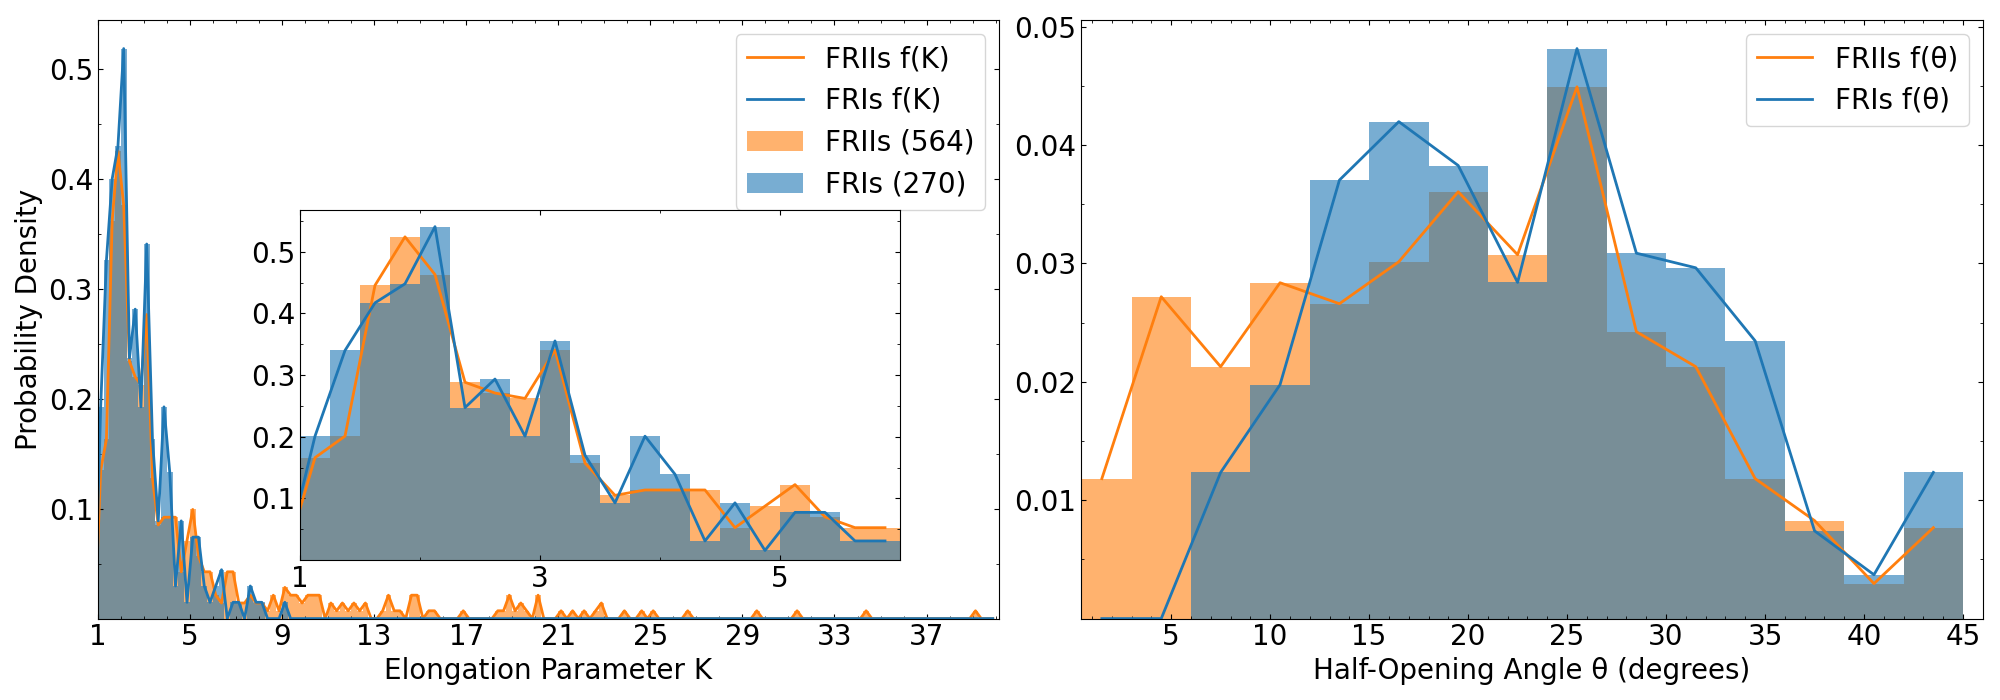
\includegraphics[width=0.9\linewidth]{Figure/Section 4/ProbabilityDensity.png}
    \caption{Left Panel: Probability density distribution of the elongation parameter K; The horizontal axis represents K, and the vertical axis denotes the probability density of K; Histogram bins for K are set at intervals of 0.25, with the corresponding curve $f(K)$ representing the probability density function of K; Red and blue colors correspond to FRIs and FRIIs, respectively. Right Panel: Probability density distribution of the half-opening angles ($\theta$) of RGs estimated using K; The horizontal axis represents the $\theta$, and the vertical axis denotes the probability density of the $\theta$; Histogram bins for the $\theta$ are set at intervals of $3^\circ$ , with the corresponding curve $f(\theta)$ representing the probability density function of the $\theta$.}
    \label{fig:Figure14}
\end{figure*}
% \clearpage


\section{Discussion}\label{sec:Discussion}

\subsection{The Deviations in Procedure}\label{sec:Section5_1}
% 大概介绍一下对源处理的偏差
% 1.光学对应体匹配
In practice, genuine optical counterparts may remain unmatched due to observational limitations. Consequently, a substantial fraction of RGs lacking matched optical counterparts must be excluded from our program. The matching status of optical counterparts is illustrated in \autoref{fig:Figure15}.
% ——要绘制图片展示匹配的光学对应体数目：1，多，0。然后讨论一下和Data中FIRST匹配数据的偏差。
\begin{figure}
    \centering
    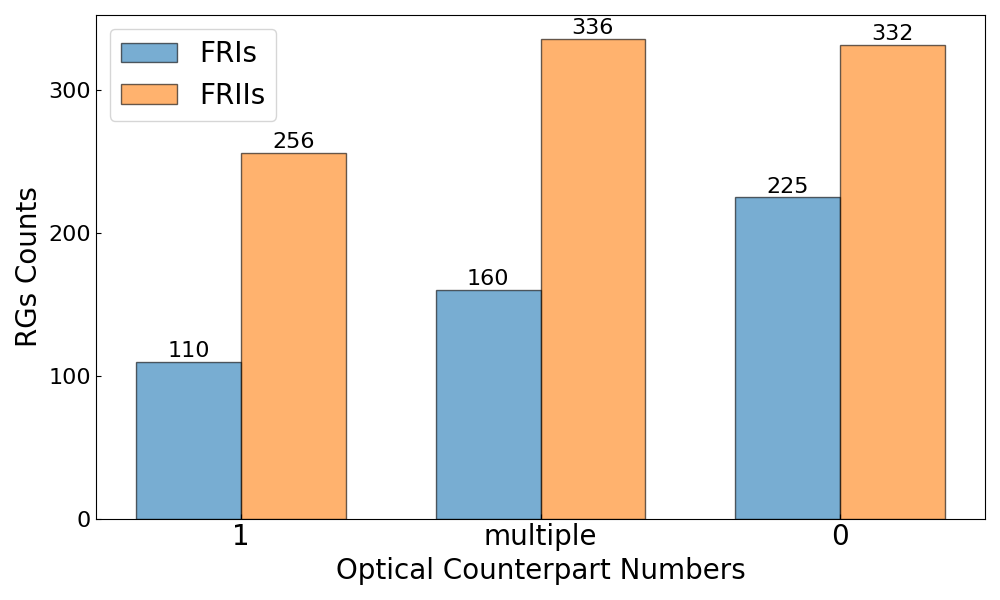
\includegraphics[width=0.9\linewidth]{Figure/Section 5/OpticalCounterpartCountDistributions.png}
    \caption{This figure illustrates the distribution of RGs during the search for their optical counterparts. The two colored labels correspond to FRI/FRII type RGs, respectively. The horizontal axis represents the number of optical counterparts detected for each RG: optical counterparts with a detection count of 1 are relatively more reliable than those with a count of "multiple", and RGs with an optical counterpart count of 0 will be excluded from our subsequent analysis. The vertical axis denotes the number of RGs.}
    \label{fig:Figure15}
\end{figure}


% 2.argue一下星系倾角问题！从各向同性出发，参考其他人的文章。
In observational studies of radio galaxies, the inclination angle problem has long been a core challenge plaguing astronomers. The inclination angle is defined as the angle between the axis of symmetry of a radio galaxy and the observer’s line of sight, and this seemingly straightforward geometric parameter actually encapsulates highly complex physical information. Since the observed radio galaxy images are essentially the projection of three-dimensional structures onto the two-dimensional celestial sphere, different inclination angles can result in entirely distinct observed morphologies for the same intrinsic structure \citep{reynolds_projection_1980}. The degeneracy arising from this projection effect renders the extraction of true physical parameters from observational data extremely challenging. With the continuous advancement of technology, several methods based on isotropy to infer the inclination angle have emerged \citep[e.g.,][]{schmitt_jet_2001,drouart_jet_2012,oei_discovery_2022}., but these approaches impose non-trivial requirements on observational data and telescope resolution\textemdash requirements that are not easily satisfied in the work presented in this paper.

% 3.高斯椭圆的结构其实也有问题
Additionally, Gaussian elliptical fitting for component extraction requires attention. With fewer constraints, its fitting accuracy may decrease, necessitating extensive manual inspection to identify poor fits and ensure high-quality source extraction. Thus, complex Gaussian fitting is unsuitable for large-scale survey data analysis; it may even cause catastrophic errors when applied to highly distinct RGs. However, it remains adequate for component extraction in simple scenarios. Notably, when constraining component division for RGs, we adopted a strict 95\% brightness threshold for FRIIs but only 80\% for FRIs. This is due to the general characteristics of FR types: FRIs often have faint, diffuse edge structures that severely hinder key region identification, whereas the more regular structure of FRIIs allows for stricter constraints. There may be cases of failure to match an ellipse. The difference in the number of FRIIs in \autoref{fig:Figure12} is precisely because some RGs cannot achieve 95\% coverage by an ellipse due to their diffuse structures. However, this issue is alleviated when the coverage threshold is reduced.


% 4.中心线定位并不准确
In this study, the BSF is utilized to locate the center line; however, this method may introduce deviations. Specifically, this localization process is analogous to pruning, which tends to eliminate "extraneous branches" in regions with complex structures. Naturally, the structural features exhibited in complex regions undergo a more pronounced simplification than those in simple regions. Our method demonstrates advantages over ridge line-based approaches: specifically, the quality of ridge lines is highly dependent on image preprocessing steps, and they are less suitable for RG systems featuring large gaps or curved head-tail structures \citep[e.g.,][]{barkus_application_2021,clews_radio-loud_2025}.



% 介绍堆叠曲线在一定区域内不可靠的情况
% Additionally, given that FRII sources typically have dim or absent core regions relative to their lobes, combined with the scarcity of large-scale data, the brightness-stacked profiles near core regions and in outer large-scale lobes are unreliable. For instance, the profiles of FRIIs exhibit obvious abrupt linear transitions around 1 kpc in their central regions\textemdash a phenomenon attributed to the fact that the brightness\textemdash distance grid near these transition sites is smaller than the pixel resolution of FIRST.


In our previous work, we have conducted research on the distribution characteristics of RGs. It can be noted that both the redshift distribution in \autoref{fig:Figure3} and mass distribution in \autoref{fig:Figure4}, the RGs exhibit concentrated clustering characteristics, with individual sources showing significant deviation from the primary cluster; however, ignoring extreme objects and considering the overall pattern, the distribution range of FRIIs is distinctly broader than that of FRIs. In terms of redshift distribution, FRIs are largely confined to regions below $z \sim 0.5$, while FRIIs extend smoothly from $z \sim 0$ to approximately $z \sim 1.5$. This likely indicates that FRIs, being intrinsically dimmer than FRIIs, are detectable only at relatively low redshifts. Regarding mass distribution, the ranges of central black hole mass and stellar mass for FRIIs are wider than those for FRIs, yet their distribution peaks are notably similar: Central black hole masses cluster near $10^{8.5} M_\odot$, and stellar masses cluster near $10^{11.5} M_\odot$. These deviations may arise from the sensitivity characteristics of telescope observations or could indeed reflect inherent differences in the physical properties of these RGs.



\subsection{Similar Mechanism of Morphological Evolution?}\label{sec:Section5_2}
% 提及应用前景
The original objective of this project is to extract statistical parameters that can characterize the structure of RGs from the sample distributed at 1.4 GHz. The Murchison Widefield Array has presented deep-exposure images of EoR in specific sky fields \citep{offringa_parametrizing_2016}, and has also demonstrated the existence of dense extragalactic sources. Such extragalactic sources serve not only as the observational background for the 21 cm forest but also may act as foreground contaminants. Once a basic understanding of such extragalactic foreground contamination is established, consideration can be given to methods for its subtraction. Some methods of foreground source modeling need subtract bright sources at the first \citep{di_matteo_radio_2002,di_matteo_21-cm_2004}.  A qualitative understanding of the structure of foreground sources is required; for example, Independent Component Analysis of \cite{chapman_foreground_2012} relies on observational constraints and physical models derived from RGs. 


% 椭圆轴比聚集于0.25，FRIs比FRIIs更弥散
To characterize the structures of RGs, we employed elliptical fitting for parameter extraction. In \autoref{sec:Section3_6}, elliptical structures can be fitted to FR-type RGs, with the axial ratios of these ellipses subsequently computed. \autoref{fig:Figure7} presents binned histograms of axial ratios for FRIs and FRIIs, constructed with the same number of bins. Although the sample size of FRIs is smaller than that of FRIIs, the overall axial ratio distribution of FRIs is considerably more dispersed. Given that FRIIs typically host more powerful central engines than FRIs, their jets may be less susceptible to environmental effects. Here, a distinct clustering in the FRII distribution is evident, suggesting that FRII radio lobe structures naturally tend toward axial ratios approaching 0.25. Notably, the peak of the FRI distribution also lies near an axial ratio of 0.25. In \autoref{fig:Figure8}, the discrepancy in physical scale distributions between FRIs and FRIIs is clearly observable and remarkably large; nevertheless, both the axial ratio and elongation parameter exhibit similar distribution patterns across the two classes. This observation implies the existence of a shared mechanism of morphological evolution in FR-type RGs.




\subsection{The Phenomenon of Brightness Stacking Curve}\label{sec:Section5_3}

% 事实上凸起不够显著，来自望远镜的偏差
First, we introduce FRIIs. The brightness stacking curve of FRIIs show brightness distribution in our study is not enough significantly compared with the pronounced protuberance observed in Turner's work. Apart from biases arising from the matching of optical counterparts and RGs, an intuitive explanation lies in observational sensitivity: the extended structures of radio AGNs may be underestimated due to insufficient sensitivity, \cite{shabala_delayed_2017} simulated model parameters for three VLBI-detected AGNs (MJV 02278, MJV 16230, and MJV 16427) and compared brightness-versus-physical-scale curves under varying telescope sensitivities to illustrate this effect.

Then we can see that the inaccuracy in centerline positioning is reflected in the stacked curves: if all identified optical counterparts of RGs could be precisely aligned with the centers of radio structures, the physical scale distribution of FRIIs in \autoref{fig:Figure13} should in principle be half of that in \autoref{fig:Figure8}. This indicates a significant deviation between the centerlines derived in this work and the optical counterparts. Potential explanations include misidentified optical counterparts for some RGs (even though we prioritized those proximate to radio structure centers as much as possible) and biases arising from the inclination angles of RGs and the Doppler effect. However, regions of substantial radio brightness adjacent to the optical counterparts are relatively reliable: Consistent with general understanding, while the radio lobes of FRIIs are brighter, their spatial distribution is random; by contrast, the faint central sources of FRIIs, when stacked together, should indeed be brighter than the lobe areas. Other prominent features can be interpreted as radio-active regions. In contrast to the distinct characteristics of FRIIs, the unilateral brightness stacking profiles of FRIs lack analogous prominent features, thus other statistical approaches for FRIs should be considered.


% 讨论一下Knots分布的故事
\subsection{The Steady Change of Knots}\label{sec:Section5_4}

Notably, for knot structures in FRIIs\textemdash such as Hot Spots describable via shock processes, and multiple Hot Spot configurations  (e.g., Double-Double radio galaxies) explainable as relics of past AGN activity\textemdash most FRIs exhibit significantly lower luminosity than FRIIs. The central engine power of FRIs is often insufficient to sustain jets at FRII-scale lengths, rendering Hot Spot models inapplicable to FRIs. Accordingly, knots are treated here as a descriptive feature for FRIs, and we shift our perspective from linear to surface-based characterizations.


Evidently, during observations, we have observed two distinct types of knots\textemdash the bright core of FRIs and the hotspots of FRIIs. However, dedicating specific discussion solely to FRII knots may not hold significant value at this point, as both double hotspots and double-double lobe configurations have already emerged as independent classification frameworks: the prevailing view regarding double-double lobes posits the potential occurrence of multiple jet outbursts, which re-energize remnants from previous outbursts, thereby forming two pairs of hotspots; additionally, the presence of more complex hotspot structures may similarly stem from multiple outbursts or limitations imposed by telescope sensitivity. In contrast to FRIIs, FRIs are fundamentally considered core-dominated in radiative luminosity, while FRII structures span a broad range from low to high brightness, whereas FRIs generally appear only in low-brightness intervals. This implies that either environmental influences prevent the establishment of bright extended structures in RGs, or the AGN power is insufficient to support extended jets interacting with the cosmic environment. Based on this a priori hypothesis, we are filled with curiosity regarding the knots observed in FRIs.


% 对nodes分布的详细介绍
In the right panel of \autoref{fig:Figure10}, the trends of the three curves (blue, black, cyan) as the brightness threshold increases reveal the characteristics of the radio brightness structures of RGs:
\begin{itemize}[label=•]
    
    \item For the blue curve (tracking node count), between ~10\% and 75\% of the peak brightness, the node count decreases relatively uniformly (the coefficient of determination for the best-fit line is ~0.96, likely due to the predominant distribution of knot brightness within this range), with minor fluctuations in the total number of nodes/knots and node-bearing RGs.
    
    \item The black curve (recording the number of RGs with recognized nodes) shows a slight decline at thresholds below 0.5\% and above 75\%—attributable to incomplete filtering of FRI systems (characterized by uniformly low luminosity and ambiguous brightness) in previous analyses—indicating that knot variation is unaffected by RG quantity. It decreases rapidly beyond 75\% because algorithmic limitations hinder the recognition of points with excessively narrow brightness ranges as nodes.
    
    \item The cyan curve (illustrating sources with only core clumps) exhibits fluctuations stemming from the "disintegration effects" of FRI core clumps—where multiple regions of non-uniform brightness gradually emerge within initially large clumps during flood-filling—and this process, alongside the discontinuous lobes around FRIs, represents the sole contributor to the node count.

\end{itemize}


% 介绍recolllimation—— knots数量真的跟recollimation无关吗？
How do AGN jets interact with their cosmic environment? A variety of physical processes regulate the dynamics and stability of these jets. As the initially overpressured jet streams away from the galactic center, its pressure decreases with increasing distance from the jet base. Eventually, it reaches a critical point where the jet pressure drops below the external environmental pressure. This pressure mismatch can cause the jet to undergo brightening—a phenomenon termed recollimation \citep[e.g.,][]{mizuno_recollimation_2015}. Furthermore, knots observed in NGC 2663 offer evidence for recollimation in FRI RGs \citep{velovic_collimation_2022}. However, in our dataset, it is clear that not all sources exhibit the trait that "more knots imply better collimation of FRI lobes." Manual inspection of our data further confirms that no correlation exists between a greater number of nodes and improved collimation of RG structures.




\section{Conclusions and Future} \label{sec:Conclusions and Future}

\subsection{Conclusions}\label{sec:Conclusions}

The objective of this work is to integrate existing research methodologies to conduct a deeper geometric analysis of RG structures based on FR-classified 1.4 GHz images.

The prevailing perspective on jets and radio lobes predominantly attributes their physics to shock-initiated processes. Within this consensus, we propose that elliptical geometries can effectively characterize FR-classified RGs. To derive optimally constrained elliptical structures, we employed Flood-filling algorithms, optical counterpart matching, and center-line construction, ultimately generating tailored elliptical models for FRI and FRII morphologies. Crucially, our methodology aims to develop a universal framework adaptable to diverse RG shapes, not limited to ellipsoidal forms. Consequently, we identified four distinct descriptive perspectives for RGs in the discussion section.


Our analysis can be summarised as follows:

\begin{itemize}[label=$\star$]

    \item From our perspective, we performed a statistical analysis on the geometric morphology of RGs, including their ellipticity axis ratio, physical scale, elongation parameter, and estimated half-opening angle. Besides refreshing our understanding of FR types, this study further quantitatively reaffirms the differences between FR I and FR II.
    
    \item The second perspective concerns the enumeration of knots in FRIs. Compared to the hotspots triggered by the relatively more powerful central engines of FRIIs, FRIs, despite their dimmer nature, also exhibit knots to a certain extent, though the role of these knots appears less significant. However, during the statistical analysis of knots, we observed that the number of knots within specific brightness intervals achieves a remarkable equilibrium, decreasing overall at a steady rate.
    
    \item Subsequently, we employed the classical $r_s$ method to analyze the sample, noting that FRIIs exhibit a substructure in the region where $r_s$ < 0.4, which arises from the significant outflow effects occurring at the hot spot.
    
    \item Finally, brightness stacked profiles. By leveraging the requirement to locate optical counterparts, we derived a curve describing both geometric and brightness characteristics of RGs—namely, the center line. Subsequently, stacking the brightness distributions of center lines from a sufficient sample size naturally reveals the average radiatively active regions. FRIIs demonstrate that average luminosity initially increases with physical scale, peaks, then decreases monotonically\textemdash a characteristic aligning closely with \cite{turner_energetics_2015} predicted dynamical model for FRIIs.
    
\end{itemize}

Integrating these perspectives collectively, this work provides improved clarity on the structural properties and evolutionary mechanisms of FR-classified RGs.




\subsection{Future}\label{sec:Future}

Future research should prioritize developing additional theoretical frameworks to explore the significant commonalities between FR I and FR II type RGs, which will substantially deepen the understanding of large-scale jet structures. A key direction lies in identifying the most critical parameters to establish a more authoritative classification system for RGs. Moreover, existing quantitative analyses under the FR classification framework remain superficial, so future progress must rely on more robust theoretical models and high-sensitivity observations targeting large-scale radio structures as foundational support to gain clearer insights into their intrinsic nature.


This work is anticipated to undergo further development and support simulation efforts in future research, including modeling jet structures for different RGs to refine the authentic jet-lobe morphologies observed by various telescopes. Furthermore, radio lobe structures may exhibit relevant interactions with the interstellar medium or intracluster medium; the description of these structures can be used to characterize the interactions between jets and the medium, and also reflect the kinematic components of the intergalactic medium as well as the characteristics of host galaxies. Additionally, special types of RGs will also be key research directions in the future, such as Giant RGs and Hybrid Morphology RGs.

%Additionally, the fine sub-kiloparsec scale structures of radio-quiet AGNs \citep[e.g., those detected in J0802+4643][]{vardoulaki_fr-type_2021} can fill the statistical gaps in this work, and the development of future radio telescopes will further expand the understanding of RG structures.


% 另外，曾经考虑过将连续中心线参数化，变为一组可描述射电结构的参数，但由于中心线定位并不清晰，用参数化描述的结果并不好
% ——强烈的核活动也会影响星际介质和星际电介质的星形成历史及其特性，从而成为它们宿主及其大尺度环境演化的基本成分。

\bibliographystyle{aa.bst}
\bibliography{BibDir/Introduction.bib,BibDir/Data,BibDir/Method,BibDir/Discussion}
% \bibliography{BibDir/Introduction.bib}
\begin{appendix}
\section{Alternative thread identification}\label{app:Alt} 




\end{appendix}






\end{document}

